\documentclass[11pt,a4paper]{article}
\usepackage[utf8]{inputenc}
\usepackage[T1]{fontenc}
\usepackage{lmodern}
\usepackage[margin=2.2cm]{geometry}
\usepackage{amsmath,amssymb}
\usepackage{booktabs,float,graphicx,xcolor,caption,subcaption,enumitem}
\usepackage{listings}
\usepackage{fancyhdr}
\usepackage{array,adjustbox}
\usepackage{tikz}
\usetikzlibrary{arrows.meta,positioning}
\usepackage[colorlinks=true,linkcolor=blue!50!black,urlcolor=blue!50!black,citecolor=blue!50!black]{hyperref}
\graphicspath{{results/figures/}}
\setlength{\parskip}{3pt}
\setlist{nosep,leftmargin=1.4em}
\captionsetup{font=small,labelfont=bf}
\renewcommand{\arraystretch}{1.08}

\lstdefinestyle{py}{language=Python,basicstyle=\ttfamily\fontsize{6.4}{7.4}\selectfont,keywordstyle=\color{blue!60!black},
  commentstyle=\color{gray},stringstyle=\color{red!50!black},showstringspaces=false,breaklines=true,
  numbers=left,numberstyle=\tiny\color{gray},numbersep=4pt,frame=single,rulecolor=\color{black!25},
  extendedchars=true,literate={→}{{$\rightarrow$}}1,columns=fullflexible,keepspaces=true,xleftmargin=10pt}
\newcommand{\src}[1]{\subsection*{\texttt{\detokenize{#1}}}\lstinputlisting[style=py]{#1}\vspace{2pt}}

% AUTO-GENERATED by make_tables.py -- do not edit
\newcommand{\vioExitVio}{1.33}
\newcommand{\vioExitGps}{2.83}
\newcommand{\vioExitVo}{4.76}
\newcommand{\vioExitImu}{35}
\newcommand{\vioRmseVio}{0.59}
\newcommand{\vioDriftPct}{0.47}
\newcommand{\vioSigmaTunnel}{1.01}
\newcommand{\vioInThreeSigma}{100}
\newcommand{\vioTunnelRmse}{0.86}
\newcommand{\slamIcp}{28.2}
\newcommand{\slamNdt}{0.46}
\newcommand{\slamLoop}{0.15}
\newcommand{\slamIcpYaw}{24}
\newcommand{\slamMapOdom}{0.249}
\newcommand{\slamMapLoop}{0.077}
\newcommand{\slamLoops}{32}
\newcommand{\slamDegTun}{0.026}
\newcommand{\slamDegOut}{0.225}
\newcommand{\slamDegRatio}{9}
\newcommand{\hdNdtLon}{1.4}
\newcommand{\hdNdtLat}{0.8}
\newcommand{\hdPfLon}{3.4}
\newcommand{\hdPfLat}{1.6}
\newcommand{\hdNdtMax}{12}
\newcommand{\hdGlobOk}{1}
\newcommand{\hdMapPts}{30\,498}
\newcommand{\btOk}{296}
\newcommand{\fsmFullOk}{298}
\newcommand{\fsmBasicOk}{142}
\newcommand{\fsmNoRecheckOk}{149}
\newcommand{\btAborts}{20}
\newcommand{\btNodes}{26}
\newcommand{\fsmTrans}{38}
\newcommand{\hyPerp}{6/6}
\newcommand{\hyPar}{4/6}
\newcommand{\hyK}{6/6}
\newcommand{\hyParTime}{13.7}
\newcommand{\hyParErr}{15}
\newcommand{\latQuinticOk}{16/20}
\newcommand{\latLinearOk}{0/20}
\newcommand{\latQuinticK}{0.075}
\newcommand{\latLinearK}{0.67}
\newcommand{\kappaMax}{0.212}
\newcommand{\slotOkA}{0/6}
\newcommand{\slotOkB}{1/6}
\newcommand{\slotOkC}{5/6}
\newcommand{\slotOkD}{6/6}
\newcommand{\slotOkE}{6/6}
\newcommand{\spdBaseOk}{4/6}
\newcommand{\spdBaseTime}{19.8}
\newcommand{\spdBaseExp}{14376}
\newcommand{\spdWaOk}{2/6}
\newcommand{\spdWaTime}{12.7}
\newcommand{\spdWaExp}{8520}
\newcommand{\spdWbOk}{2/6}
\newcommand{\spdWbTime}{11.3}
\newcommand{\spdWbExp}{7504}
\newcommand{\spdDubOk}{4/6}
\newcommand{\spdDubTime}{22.2}
\newcommand{\spdDubExp}{17949}
\newcommand{\lfFail}{4}
\newcommand{\lfSolvZero}{0}
\newcommand{\lfSolvMargin}{0}
\newcommand{\lfRecovered}{0}
\newcommand{\lfOkUnsolv}{1}
\newcommand{\sensSlamLoop}{0.13 [0.10, 0.17]}
\newcommand{\sensSlamOdom}{0.35 [0.26, 0.44]}
\newcommand{\sensSlamIcp}{29.4 [27.4, 31.4]}
\newcommand{\sensNdtNom}{1.7 [1.6, 1.9]}
\newcommand{\sensPfNom}{3.8 [3.7, 4.0]}
\newcommand{\sensSeeds}{20}
\newcommand{\sensNdtNoise}{4.4 [4.2, 4.6]}
\newcommand{\sensPfNoise}{4.4 [4.2, 4.6]}
\newcommand{\sensNdtNoiseFail}{1/20}
\newcommand{\sensNdtDrop}{2.7 [2.5, 2.8]}
\newcommand{\sensPfDrop}{3.8 [3.7, 4.0]}
\newcommand{\sensNdtDropFail}{0/20}
\newcommand{\clGt}{10/10}
\newcommand{\clNdt}{10/10}
\newcommand{\clDr}{0/10}
\newcommand{\clNdtLoc}{3.1}
\newcommand{\clDrLoc}{0.62}
\newcommand{\clCte}{0.15}
\newcommand{\clClrNdt}{0.48}
\newcommand{\clClrGt}{0.50}
   % headline numbers, auto-generated (python make_tables.py)

\title{Localization, Mapping and Motion Planning for a Self-Driving Car:\\[2pt]
\large A Simulation Study of Visual-Inertial Odometry, LiDAR SLAM, HD-Map Localization,\\ Behaviour Trees and Hybrid~A*}
\author{\href{mailto:vishwasnarayan2345@gmail.com}{vishwasnarayan2345@gmail.com}}
\date{November 2026}

\pagestyle{fancy}\fancyhf{}
\fancyhead[L]{\small\itshape Localization, Mapping and Planning for Self-Driving Cars}
\fancyhead[R]{\small\thepage}
\renewcommand{\headrulewidth}{0.3pt}
\fancypagestyle{plain}{\fancyhf{}\fancyfoot[C]{\small\thepage}\renewcommand{\headrulewidth}{0}}

\begin{document}
\begin{titlepage}
\centering\vspace*{2.2cm}
{\large Project report (M.Tech level)\par}\vspace{1.4cm}
{\Large\bfseries Localization, Mapping and Motion Planning\\ for a Self-Driving Car\par}\vspace{0.5cm}
{\large Visual-inertial odometry $\cdot$ LiDAR SLAM $\cdot$ HD-map localization\\ Behaviour trees $\cdot$ Hybrid~A* and state lattices\par}\vspace{1.6cm}
{\large\href{mailto:vishwasnarayan2345@gmail.com}{vishwasnarayan2345@gmail.com}\par}\vspace{0.4cm}
{\large November 2026\par}\vfill
\begin{minipage}{0.85\linewidth}\small\noindent
\textbf{Status.} Nine simulation experiments are complete (E1--E5 core, E6--E9 extended) and reported with measured numbers (Section~\ref{sec:results}). Experiments planned for the coming weeks, and a longer list of research ideas, are in Section~\ref{sec:future}. All code and raw results are in the accompanying folder (Section~\ref{sec:repro}); \texttt{python run\_all.py} regenerates every number, figure and table in this report.
\end{minipage}\vspace{1.5cm}
\end{titlepage}

\begin{abstract}\noindent
Safe automated driving needs a vehicle that knows where it is, decides sensibly and moves along paths it can physically drive. This report studies five building blocks of such a stack in a reproducible 2-D urban simulation, implemented from scratch in NumPy/SciPy:
(i)~a visual-inertial odometry (VIO) filter that bridges GPS outages in a tunnel and an underpass, (ii)~LiDAR SLAM with NDT registration and pose-graph loop closure, (iii)~localization against a pre-built HD map with NDT and a particle filter, (iv)~behaviour trees (BT) for overtaking, roundabout and pedestrian yielding compared with finite-state machines (FSM), and (v)~Hybrid~A* and a Frenet state lattice for kinematically feasible paths.
Measured results: VIO tunnel-exit error \vioExitVio\,m against \vioExitGps\,m without vision (20 seeds); NDT+loop-closure SLAM ATE \slamLoop\,m against \slamIcp\,m for scan-to-scan ICP; HD-map NDT localization at \hdNdtLon/\hdNdtLat\,cm (lon/lat RMS); BT \btOk/300 scenarios against \fsmFullOk/300 for a complete FSM and \fsmBasicOk/300 for a basic one; Hybrid~A* feasible in \hyPerp\ perpendicular, \hyPar\ parallel and \hyK\ K-turn trials where grid~A* produced no feasible path.
Extended runs add a Hybrid~A* slot-length sweep, a 20-seed statistical study of SLAM and HD-map localization, a lattice failure analysis and a closed-loop run in which NDT localization drives the whole stack (\clNdt\ successes) while VO dead reckoning fails (\clDr).
The study is simulation-only, uses simulated visual odometry and, for most experiments, a small number of seeds; Section~\ref{sec:limits} states what the results do \emph{not} show, and Section~\ref{sec:future} lists the follow-up experiments.
\par\medskip\noindent\textbf{Keywords:} visual-inertial odometry, LiDAR SLAM, normal distributions transform, particle filter, HD map, behaviour trees, Hybrid A*, state lattice, autonomous driving.
\end{abstract}

\tableofcontents
\listoffigures
\listoftables
\clearpage

\section{Introduction}
\subsection{Motivation and problem statement}
An automated vehicle has to answer three questions continuously: \emph{where am I?} (localization and mapping), \emph{what should I do?} (behaviour decision) and \emph{how do I get there?} (motion planning). Each has a well-known failure mode: GNSS is unavailable in tunnels and urban canyons; odometry and scan-matching drift; maps become stale; hand-wired decision logic becomes brittle as behaviours are added; and grid-based paths ignore the vehicle's minimum turning radius and body shape. This project builds one working implementation of a remedy for each and measures how well it works, on a common simulator, with fixed seeds.

\subsection{Objectives}
\begin{itemize}
\item \textbf{O1} Keep a metre-level position estimate through GPS-denied tunnel and underpass sections (VIO).
\item \textbf{O2} Build a consistent map online and quantify drift with and without loop closure (LiDAR SLAM).
\item \textbf{O3} Localize to centimetre level against a pre-built HD map and test robustness to unmapped objects (NDT, particle filter).
\item \textbf{O4} Replace a rigid FSM by a BT for overtaking, roundabout yielding and pedestrian yielding, and measure the trade-off.
\item \textbf{O5} Generate smooth, curvature-bounded paths for parking and tight turns (Hybrid~A*) and for on-road obstacle avoidance (state lattice), against grid-based baselines.
\end{itemize}

\subsection{Contributions}
\begin{enumerate}[label=\textbf{C\arabic*}]
\item A compact code base (about 3\,700 lines of Python for library, experiments and tests) implementing a stochastic-cloning VIO EKF, multi-resolution NDT SLAM with an SE(2) pose graph, HD-map NDT and particle-filter localization, a behaviour-tree library with FSM baselines, and Hybrid~A* with Dubins shots and a quintic Frenet lattice.
\item A reproducible simulation benchmark with GPS-denied sections, repetitive geometry, unmapped objects, scripted traffic scenarios and tight parking maps; every experiment is seeded and regenerates its figures and LaTeX tables.
\item Nine experiments with measured results, including the cases that did \emph{not} work: global localization converged in \hdGlobOk\ of 3 seeds, parallel parking was solved in \hyPar\ trials, search speed-ups lost solutions, and a complete FSM matched the BT in safety (the BT advantage found is structural).
\item An explicit validity analysis and a list of planned experiments and research ideas (Section~\ref{sec:future}).
\end{enumerate}
\textbf{Scope.} Planar (SE(2)) models, one synthetic map, modules evaluated independently (no closed loop yet). The ``visual'' front end is \emph{not} implemented: VO measurements are simulated from ground truth with a parametric error model.

\section{Related work}
\textbf{Visual-inertial odometry.} Filter-based VIO such as the MSCKF~\cite{mourikis07} keeps a window of camera poses in the state; stochastic cloning~\cite{roumeliotis02} is the underlying device for processing relative-pose measurements without double counting. Optimization-based systems (OKVIS~\cite{leutenegger15}, VINS-Mono~\cite{qin18}, ORB-SLAM3~\cite{campos21}) use IMU preintegration~\cite{forster17}. The filter here follows the first line in a loosely coupled, planar form.

\textbf{LiDAR odometry and SLAM.} Scan-to-scan ICP~\cite{besl92,segal09} drifts; LOAM~\cite{zhang14} and its descendants~\cite{shan18,shan20,xu22} register edge and planar features to a local map. The normal distributions transform (NDT)~\cite{biber03,magnusson09} registers a scan to a grid of Gaussians and is the basis of HDL-graph-SLAM~\cite{koide19}. Back ends are pose graphs~\cite{grisetti10,kummerle11}; loop edges are commonly robustified (Huber~\cite{huber64}, switchable constraints~\cite{sunderhauf12}). Degeneracy of the registration problem (e.g.\ corridors) can be read from the Hessian spectrum~\cite{zhang16}, which motivates the indicator used here.

\textbf{Map-based localization.} Monte Carlo localization~\cite{dellaert99} and NDT matching against a prior point-cloud map are the two standard approaches in open-source driving stacks~\cite{kato18}; HD-map formats such as Lanelet2~\cite{poggenhans18} add semantics. Probabilistic foundations are in~\cite{thrun05}.

\textbf{Behaviour architectures.} FSMs are the traditional choice; behaviour trees~\cite{colledanchise18,iovino22} provide hierarchy, reactivity and modularity and are used in robot navigation stacks~\cite{macenski20}. Quantitative FSM-versus-BT comparisons on driving scenarios are rare, which motivates E4.

\textbf{Motion planning.} Hybrid~A*~\cite{dolgov10} searches continuous vehicle states on a discretized grid; Dubins~\cite{dubins57} and Reeds--Shepp~\cite{reeds90} curves give analytic connections and heuristics; state lattices~\cite{pivtoraiko09} and Frenet-frame polynomial sampling~\cite{werling10} are the on-road counterparts. Optimization-based refinement~\cite{zhang21} and production planners~\cite{fan18} build on these. Surveys: \cite{paden16}.

\section{Problem formulation and evaluation metrics}\label{sec:formulation}
\textbf{Notation.} A planar pose is $\mathbf{x}=(\mathbf{p},\theta)\in SE(2)$, $\mathbf{p}\in\mathbb{R}^2$, with rotation $R(\theta)$; $\oplus$ composes and $\ominus$ gives the relative pose. Inputs are IMU samples $(g_z,\mathbf{a}_m)$, relative visual odometry $\mathbf{z}_{vo}$, intermittent GPS positions $\mathbf{z}_{gps}$, 2-D LiDAR scans $\mathcal{S}_k$ and, for E3, a map $\mathcal{M}$. The estimation task is $\hat{\mathbf{x}}_k=f(\text{inputs}_{1:k})$.

\textbf{Localization errors.} With ground truth $\mathbf{x}^{gt}$ and $\mathbf{d}=\hat{\mathbf{p}}-\mathbf{p}^{gt}$,
\begin{equation}
\begin{bmatrix}e_{lon}\\e_{lat}\end{bmatrix}=R(\theta^{gt})^{\!\top}\mathbf{d},\qquad e_{pos}=\|\mathbf{d}\|,\qquad
\mathrm{ATE}=\sqrt{\tfrac1N\sum_{i=1}^{N}\|\hat{\mathbf{p}}_i-\mathbf{p}^{gt}_i\|^2}.
\end{equation}
All estimators start from the known initial pose, so no trajectory alignment is applied before computing ATE~\cite{sturm12,zhang18}. SLAM ATE is evaluated at keyframes; map error is the nearest-neighbour distance from map points to noise-free simulator geometry.

\textbf{Decision metric.} A scenario is a \emph{success} if the ego vehicle reaches the end of the route without collision. Hard-brake events and structural size (nodes, transitions) are reported as secondary metrics.

\textbf{Planning feasibility.} A path is \emph{feasible} if it (a) is collision-free for the exact rectangular footprint, (b) has peak curvature $\le1.05\,\kappa_{\max}$, and (c) ends within 0.35\,m and $6^\circ$ of the goal pose (parking) --- for the lattice, (a) and (b) only. The search itself accepts a goal within 0.30\,m and 0.09\,rad.

\textbf{Reporting.} Means $\pm$ sample standard deviations are over seeds; no significance tests are run because sample sizes are small (3--20 seeds).

\section{System architecture and code layout}
\begin{figure}[H]\centering
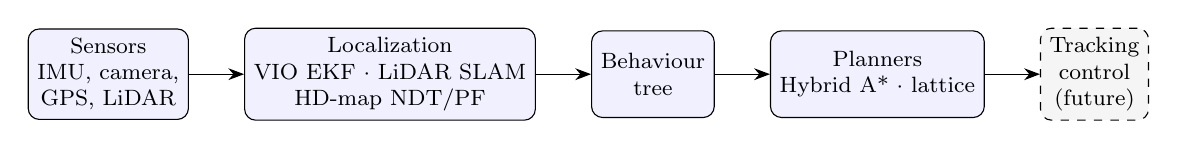
\begin{tikzpicture}[node distance=7mm,box/.style={draw,rounded corners,align=center,minimum height=1.1cm,font=\footnotesize,fill=blue!6},
  fut/.style={box,dashed,fill=gray!8},>={Stealth[length=2mm]}]
\node[box](s){Sensors\\IMU, camera,\\GPS, LiDAR};
\node[box,right=of s](l){Localization\\VIO EKF $\cdot$ LiDAR SLAM\\HD-map NDT/PF};
\node[box,right=of l](b){Behaviour\\tree};
\node[box,right=of b](p){Planners\\Hybrid A* $\cdot$ lattice};
\node[fut,right=of p](c){Tracking\\control\\(future)};
\draw[->](s)--(l);\draw[->](l)--(b);\draw[->](b)--(p);\draw[->](p)--(c);
\end{tikzpicture}
\caption{Pipeline. Each solid block is implemented and evaluated on its own; integration is planned (P4).}
\end{figure}

\begin{table}[H]\centering\small
\caption{Modules and source files (full listings in Appendix~\ref{app:code}).}
\begin{tabular}{lp{7.0cm}l}\toprule
Topic & Files & Experiment\\\midrule
Simulator, sensors & \texttt{sim/world.py}, \texttt{sim/drive.py}, \texttt{geometry.py} & all\\
VIO (EKF, stochastic cloning) & \texttt{localization/vio.py} & E1\\
LiDAR SLAM (NDT, ICP, pose graph) & \texttt{ndt.py}, \texttt{icp.py}, \texttt{pose\_graph.py}, \texttt{lidar\_slam.py} & E2\\
HD map, NDT/PF localization & \texttt{hd\_map.py}, \texttt{particle\_filter.py} & E3\\
Behaviour tree, FSM baselines & \texttt{behavior/bt.py}, \texttt{behavior/scenario.py} & E4\\
Hybrid A*, Dubins, lattice & \texttt{planning/*.py} & E5\\
Unit tests & \texttt{tests/test\_core.py} (6 tests, pass) & --\\\bottomrule
\end{tabular}\end{table}

\section{Simulation environment}
The road is a closed rounded rectangle ($220\times140$\,m, corner radius 25\,m, length 677\,m) with buildings, poles and trees, a 130\,m curved \emph{tunnel} (route position $s\in[200,330]$\,m, low texture) and a 25\,m \emph{underpass} ($s\in[500,525]$\,m); GPS is unavailable in both. The vehicle drives 1.25 laps (846\,m) with a curvature-limited speed profile ($\le11$\,m/s).

\begin{table}[H]\centering\small
\caption{Sensor models (all noise parameters are in \texttt{sim/drive.py}).}
\begin{tabular}{llp{8.4cm}}\toprule
Sensor & Rate & Model\\\midrule
IMU & 100\,Hz & gyro-$z$ and body-frame $(a_x,a_y)$; white noise $0.002$\,rad/s, $0.05$\,m/s$^2$; random-walk biases\\
Visual odometry & 10\,Hz & relative pose; $\sigma_t=1\,\text{cm}+1\%\cdot d$, $\sigma_r=1.5\,\text{mrad}+0.2\%\cdot|\Delta\theta|$, 0.4\% scale error, $\times2.5$ noise in the tunnel\\
GPS & 1\,Hz & position, $\sigma=0.6$\,m, absent in tunnel/underpass\\
LiDAR & 10\,Hz & 360 beams, 40\,m range, $\sigma=2\,\text{cm}+0.1\%\cdot r$, 2\% dropout, ray-cast against walls and poles\\\bottomrule
\end{tabular}\end{table}
The HD map ($\hdMapPts$ points) is built from a separate survey drive using LiDAR scans placed with ground-truth poses perturbed by $(2\,\text{cm},2\,\text{cm},1.5\,\text{mrad})$, a stand-in for an RTK-INS mapping vehicle.

\section{Methods and implementation}
\subsection{Visual-inertial odometry (\texttt{vio.py})}
A loosely coupled EKF with state $\mathbf{x}=[\mathbf{p},\theta,\mathbf{v},b_g,\mathbf{b}_a]\in\mathbb{R}^8$ and a \emph{cloned} previous camera pose $\mathbf{c}=(\mathbf{p}_c,\theta_c)$ (stochastic cloning), so that relative VO measurements do not reuse information. IMU propagation:
\begin{equation}
\omega=g_z-b_g,\quad \mathbf{a}_w=R(\theta)(\mathbf{a}_m-\mathbf{b}_a),\quad
\mathbf{p}\!\leftarrow\!\mathbf{p}+\mathbf{v}\Delta t+\tfrac12\mathbf{a}_w\Delta t^2,\quad \mathbf{v}\!\leftarrow\!\mathbf{v}+\mathbf{a}_w\Delta t,\quad \theta\!\leftarrow\!\theta+\omega\Delta t .
\end{equation}
The VO update compares the measured relative pose with the one implied by the state and the clone, then re-clones:
\begin{equation}
\mathbf{z}_{vo}=\begin{bmatrix}R(\theta_c)^{\!\top}(\mathbf{p}-\mathbf{p}_c)\\ \theta-\theta_c\end{bmatrix}+\mathbf{n},\qquad \mathbf{n}\sim\mathcal{N}\big(0,\operatorname{diag}(\sigma_t^2,\sigma_t^2,\sigma_r^2)\big)\cdot 1.3^2 .
\end{equation}
GPS updates ($\mathbf{z}=\mathbf{p}+\mathbf{n}$) and VO updates are $\chi^2$-gated (99.9\%)~\cite{barshalom01}. The covariance uses the Joseph form and is symmetrized after every step (needed for low VO noise, where round-off otherwise made the position variance negative).

\subsection{LiDAR SLAM (\texttt{ndt.py}, \texttt{lidar\_slam.py}, \texttt{pose\_graph.py})}
\textbf{Front end} (HDL-graph-SLAM style~\cite{koide19}, NDT~\cite{biber03}): keyframe-based NDT scan-to-submap registration (last 20 keyframes, cells 3\,m then 1.5\,m, four half-cell-shifted grids). With $\mathbf{x}'_i=T(\mathbf{p})\mathbf{x}_i$ and cell mean/covariance $(\boldsymbol\mu_i,\Sigma_i)$ the cost minimised by damped Newton is
\begin{equation}
F(\mathbf{p})=\sum_i d_1\exp\!\Big(-\tfrac{d_2}{2}(\mathbf{x}'_i-\boldsymbol\mu_i)^{\!\top}\Sigma_i^{-1}(\mathbf{x}'_i-\boldsymbol\mu_i)\Big),\qquad d_1<0 ,
\end{equation}
with $d_1,d_2$ from the Gaussian-plus-uniform approximation. The conditioning of the translational Hessian block, $\rho=\lambda_{\min}/\lambda_{\max}$, is logged per scan as a degeneracy indicator.
A new keyframe is added every 1.5\,m or 0.15\,rad. \textbf{Loops} are proposed when a keyframe is within 20\,m of one that is $>80$\,m of travel away, verified by multi-start NDT with a KD-tree inlier ratio $\ge0.65$. \textbf{Back end:} SE(2) pose graph
\begin{equation}
\min_{\mathbf{x}}\sum_{(i,j)}\varrho\big(\mathbf{e}_{ij}^{\top}\Omega_{ij}\mathbf{e}_{ij}\big),\quad
\mathbf{e}_{ij}=\begin{bmatrix}R(z_\theta)^{\!\top}\big(R(\theta_i)^{\!\top}(\mathbf{t}_j-\mathbf{t}_i)-\mathbf{z}_t\big)\\ \operatorname{wrap}(\theta_j-\theta_i-z_\theta)\end{bmatrix},
\end{equation}
solved by sparse Gauss--Newton with a Huber weight $3/\sqrt{\chi^2}$ on loop edges. Baseline: scan-to-scan point-to-line ICP odometry. A LOAM-style curvature feature extractor (\texttt{extract\_loam\_features}) is implemented but \emph{not} part of E2 (see P1).

\subsection{HD-map localization (\texttt{hd\_map.py}, \texttt{particle\_filter.py})}
\textbf{NDT localizer:} the same multi-resolution NDT, registering each scan against the HD-map NDT grid from an odometry prediction (VO relative pose). \textbf{Particle filter:} 500 particles, motion noise on the VO increment, likelihood from a Euclidean distance field $d(\cdot)$ of the map with 72 beams per scan:
\begin{equation}
w^{[m]}\propto\prod_{k}\Big[(1-z_r)\,e^{-d_k^{2}/2\sigma^{2}}+z_r\Big]^{\beta},\quad \sigma=0.2\,\text{m},\ z_r=0.08,\ \beta=0.35,
\end{equation}
with systematic resampling when $N_{\text{eff}}<N/2$.

\subsection{Behaviour tree (\texttt{bt.py}, \texttt{scenario.py})}
A tick-based BT library (Sequence $\rightarrow$, Fallback ?, Condition, Action) with blackboard; a higher-priority branch \emph{halts} running lower branches (pre-emption). The decision tree (Fig.~\ref{fig:bt}) is re-evaluated every 0.1\,s: emergency brake $>$ pedestrian yield $>$ roundabout (enter if the gap is safe, else hold at the yield line) $>$ abort overtake $>$ overtake $>$ follow $>$ cruise. Longitudinal control is an intelligent-driver model (IDM)~\cite{treiber00} towards the target speed or a virtual obstacle (stop line, lead vehicle); lane changes are quintic. Two hand-written FSMs use the same predicates and controller: \emph{FSM-basic} (transitions for the nominal sequence plus a global emergency brake) and \emph{FSM-full} (adds abort and yield edges from every relevant state).
\begin{figure}[H]\centering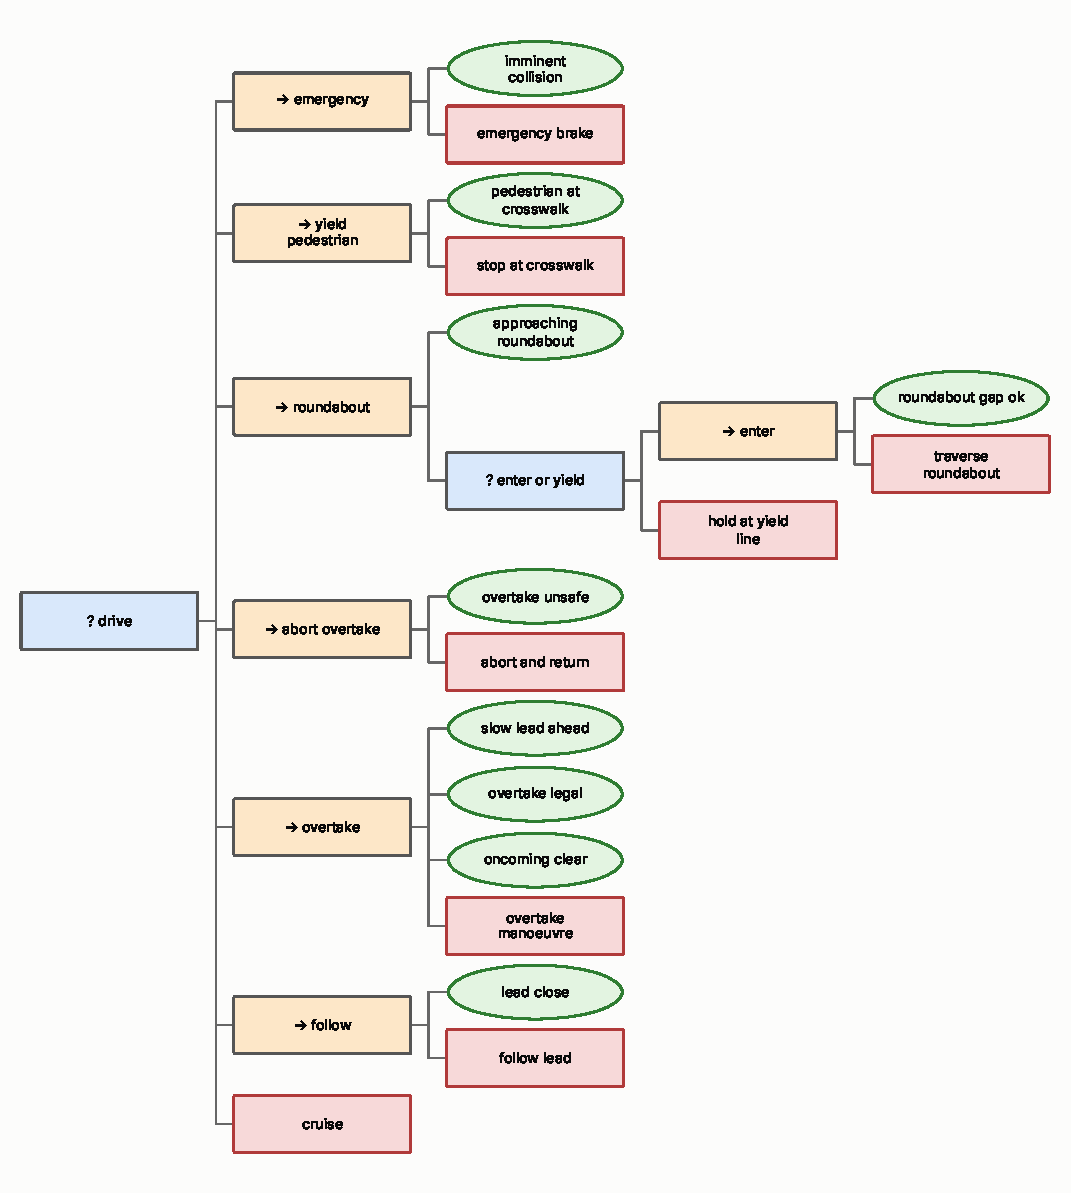
\includegraphics[width=0.88\linewidth,height=0.6\textheight,keepaspectratio]{fig_bt_tree.pdf}\caption{Implemented behaviour tree, priority from top to bottom (? = fallback, $\rightarrow$ = sequence, ellipse = condition, red box = action).}\label{fig:bt}\end{figure}

\subsection{Hybrid A* and state lattice (\texttt{hybrid\_astar.py}, \texttt{dubins.py}, \texttt{lattice.py})}
\textbf{Hybrid A*}~\cite{dolgov10} searches continuous poses of a kinematic bicycle ($\dot\theta=\tfrac{v}{L}\tan\delta$, $L=2.7$\,m, $|\delta|\le0.52$\,rad, hence $\rho_{\min}=4.72$\,m, $\kappa_{\max}=0.212$\,m$^{-1}$) with five steering angles $\times$ \{forward, reverse\} $\times$ arc lengths \{0.6, 1.5\}\,m, de-duplicated on a $0.5$\,m/$5^\circ$ grid. Arc cost
\begin{align}
\Delta g&=s\,(1+2\cdot\mathbb{1}_{rev})+0.4|\delta|+1.5|\delta-\delta_{prev}|+6\cdot\mathbb{1}_{gear\ switch},\\
h&=\max\big(h_{hol},\ \min(L_{Dubins}^{fwd},\,3L_{Dubins}^{rev})\big),
\end{align}
where $h_{hol}$ is a holonomic Dijkstra distance on the obstacle grid. A collision-checked Dubins ``shot'' (forward or time-reversed for reverse driving) to the goal is attempted during the search. The 0.6\,m arcs are needed to move inside slots that leave $\approx0.85$\,m of slack at each end. Collision checking samples the oriented car rectangle (0.3\,m lattice) on a distance field; final paths are re-verified against raw occupancy with a 4\,cm raster. \textbf{Baseline:} 8-connected grid A* for a point robot inflated by half the car width (optimistic), raw and Chaikin-smoothed~\cite{chaikin74}; both use A*~\cite{hart68}.

\textbf{State lattice} (Frenet frame of the route): quintic lateral profiles $d(s)$ with $(d_0,d_0',d_0'')\to(d_f,0,0)$ over horizons $S_f\in\{18,26,36\}$\,m and 13 terminal offsets, so the stitched receding-horizon path is $C^2$. Curvature on a road of curvature $\kappa_r$ ($\kappa_r'$ neglected):
\begin{align}
\kappa&=\frac{\kappa_r+\dfrac{d''a+d'^{2}\kappa_r}{a^2+d'^2}}{\sqrt{a^2+d'^2}},\quad a=1-\kappa_r d,\\
J&=40\!\int\! d'''^{2}ds+\big[(d_f-d_{ref})^2+\overline{(d-d_{ref})^2}\big]+200\max(|\kappa|_{\max}-0.6\kappa_{\lim},0)^2 .
\end{align}
Candidates leaving the road, exceeding $\kappa_{\lim}$ or closer than 0.35\,m to an obstacle (disc model) are rejected. The baseline uses the same candidates and checks but piecewise-linear 12\,m ramps.

\subsection{Closed-loop stack (\texttt{exp9\_closed\_loop.py})}
Every 0.1\,s a pose estimate is produced by one of three sources: ground truth, NDT against the HD map (with the simulated VO increment as prior), or VO dead reckoning. Every 0.5\,s the estimate is projected to a Frenet state $(s,d,d')$, a three-behaviour BT (\emph{stop} if the last plan had no feasible candidate, \emph{slow} at 5\,m/s if an obstacle is within 45\,m, else \emph{cruise} at 8\,m/s) sets the speed, and the quintic lattice plans around the 7 obstacles. A pure-pursuit tracker steers a kinematic bicycle (50\,Hz, steering rate $\le0.6$\,rad/s) using the \emph{estimated} pose:
\begin{equation}
\delta=\operatorname{atan2}\big(2L\sin\alpha,\;L_d\big),\qquad L_d=\operatorname{clip}(v+3,\,4,\,10)\ \text{m},
\end{equation}
with $\alpha$ the bearing of the look-ahead point relative to the estimated heading. Obstacle positions are known exactly (perfect perception) but are absent from the HD map, and are rendered as octagons in the simulated LiDAR scans, so NDT sees them as unmapped objects. A run is a success if the true body reaches $s=360$\,m without touching an obstacle.

\section{Experimental methodology}
\begin{table}[H]\centering\small
\caption{Completed experiments. Scripts are in \texttt{experiments/}; raw results in \texttt{results/*.json}.}
\begin{tabular}{llp{5.2cm}p{3.6cm}}\toprule
ID & Script & Setup & Metrics\\\midrule
E1 & \texttt{exp1\_vio.py} & 20 seeds of sensor noise; 4 estimators + VIO with GPS only for 10\,s; VO-noise sweep ($\times$0.5--4) & position RMSE, tunnel exit/max, underpass max, yaw\\
E2 & \texttt{exp2\_slam.py} & 3 seeds (drive and noise); ICP vs NDT odometry vs NDT + loops; map vs noise-free geometry & ATE (keyframes), map error, ms/scan, $\rho$\\
E3 & \texttt{exp3\_hdmap.py} & 3 seeds $\times$ {0,15,40} unmapped vehicles; PF sweep; global localization (20k particles, 3 seeds) & lon/lat/yaw RMS, P95, convergence\\
E4 & \texttt{exp4\_behavior.py} & 300 random scenarios (seed 123); BT, FSM-basic, FSM-full, FSM-full minus one edge & success, collisions, hard brakes, structure\\
E5 & \texttt{exp5\_planning.py} & 3 tight-space maps $\times$ 6 start poses; 20 random obstacle layouts for the lattice & feasibility, time, cusps, $\kappa_{\max}$\\
E6 & \texttt{exp6\_hybrid\_sweep.py} & parallel slot 5.5--7.5\,m $\times$ 6 starts; 4 search variants at 6.2\,m & feasible starts, time, expansions\\
E7 & \texttt{exp7\_lattice\_failures.py} & the 4 failing E5 layouts: Frenet-grid solvability, denser lattice, 2\,m replanning & solvable?, recovered?\\
E8 & \texttt{exp8\_sensitivity.py} & E2 with 20 seeds; E3 with 20 seeds $\times$ \{nominal, noise $\times4$, 40\% dropout\} & mean, 95\% bootstrap CI, failures\\
E9 & \texttt{exp9\_closed\_loop.py} & 3 pose sources $\times$ 10 runs through the full stack & success, clearance, cross-track\\\bottomrule
\end{tabular}\end{table}
Errors are measured against simulator ground truth. Means $\pm$ standard deviations are over seeds; E8 reports means with 95\% percentile-bootstrap confidence intervals (5\,000 resamples). Seeds are fixed in the scripts, so every number can be regenerated with \texttt{python run\_all.py}.

\section{Results (completed experiments)}\label{sec:results}
\subsection{E1: VIO through GPS-denied sections}
\begin{figure}[H]\centering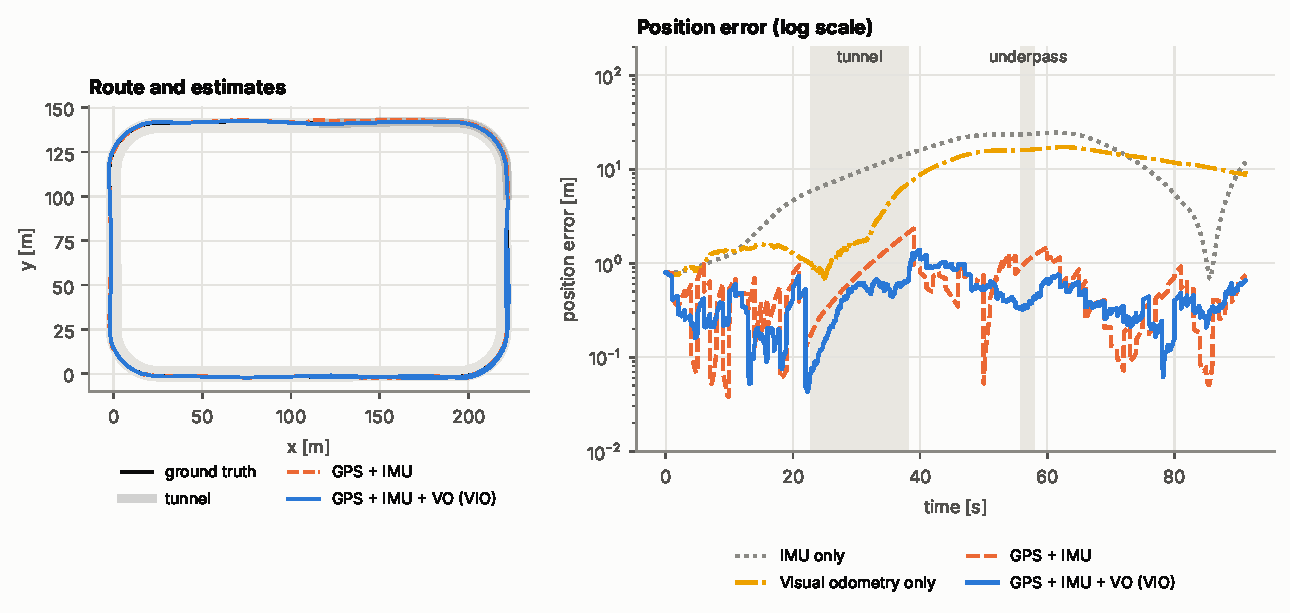
\includegraphics[width=\linewidth]{fig_vio_overview.pdf}
\caption{E1, representative run. Left: route (tunnel in grey). Right: position error (log scale); shaded = tunnel and underpass.}\label{fig:vio}\end{figure}
\begin{figure}[H]\centering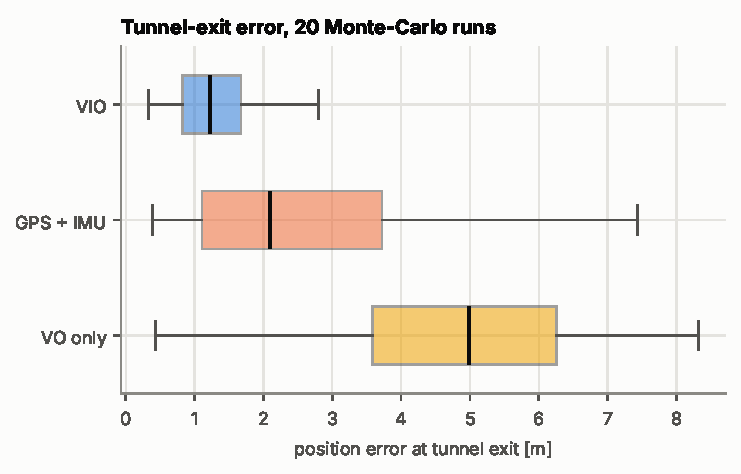
\includegraphics[width=0.5\linewidth]{fig_vio_exit_box.pdf}\caption{E1: tunnel-exit error across the Monte-Carlo runs.}\end{figure}
Tunnel-exit error is \vioExitVio\,m for VIO, against \vioExitGps\,m for the same EKF without VO, \vioExitVo\,m for VO alone and \vioExitImu\,m for the IMU alone (Table~\ref{tab:vio}); VIO whole-run RMSE is \vioRmseVio\,m. If GPS is removed after 10\,s, the final error is \vioDriftPct\% of the distance driven. In the tunnel the filter reports $\sigma\approx\vioSigmaTunnel$\,m (radial) against a measured RMSE of \vioTunnelRmse\,m, and errors stay inside $3\sigma$ for \vioInThreeSigma\% of tunnel samples, so the covariance is conservative rather than over-confident. Exit error grows monotonically with VO noise (Table~\ref{tab:vio_sweep}).
\textbf{Observation:} VIO gives \emph{metre-level} continuity during outages; centimetre level comes only from map-based localization (E3). The VO input is simulated, so these numbers bound the filter, not a real camera pipeline.
% AUTO-GENERATED by make_tables.py
\begin{table}[H]\centering\small
\caption{E1: position error [m] over a 1.25-lap drive (20 Monte-Carlo runs, mean$\pm$std).}\label{tab:vio}
\begin{adjustbox}{max width=\linewidth}
\begin{tabular}{lrrrrr}\toprule
Estimator & RMSE & Max in tunnel & Tunnel exit & Max underpass & Yaw RMSE [deg] \\ \midrule
IMU only & 43.48$\pm$23.65 & 35.40$\pm$19.96 & 35.40$\pm$19.96 & 58.92$\pm$34.34 & 12.13 \\
Visual odometry only & 6.66$\pm$2.84 & 5.26$\pm$2.09 & 4.76$\pm$2.25 & 8.71$\pm$4.81 & 2.31 \\
GPS + IMU & 0.97$\pm$0.40 & 2.92$\pm$2.03 & 2.83$\pm$2.11 & 0.75$\pm$0.33 & 1.30 \\
GPS + IMU + VO (VIO) & 0.59$\pm$0.17 & 1.42$\pm$0.72 & 1.33$\pm$0.74 & 0.62$\pm$0.27 & 0.54 \\
VIO, GPS only first 10\,s & 3.12$\pm$1.56 & 2.77$\pm$1.16 & 2.57$\pm$1.19 & 4.41$\pm$2.38 & 1.45 \\
\bottomrule\end{tabular}\end{adjustbox}
\end{table}

% AUTO-GENERATED by make_tables.py
\begin{table}[H]\centering\small
\caption{E1: VIO tunnel-exit error vs.\ VO noise scale (6 runs each).}\label{tab:vio_sweep}
\begin{adjustbox}{max width=\linewidth}
\begin{tabular}{lrrrr}\toprule
VO noise scale & $\times$0.5 & $\times$1.0 & $\times$2.0 & $\times$4.0 \\ \midrule
Tunnel-exit error [m] & 0.84 & 1.49 & 2.34 & 3.42 \\
Max tunnel error [m] & 0.88 & 1.54 & 2.39 & 3.44 \\
\bottomrule\end{tabular}\end{adjustbox}
\end{table}


\subsection{E2: LiDAR SLAM}
\begin{figure}[H]\centering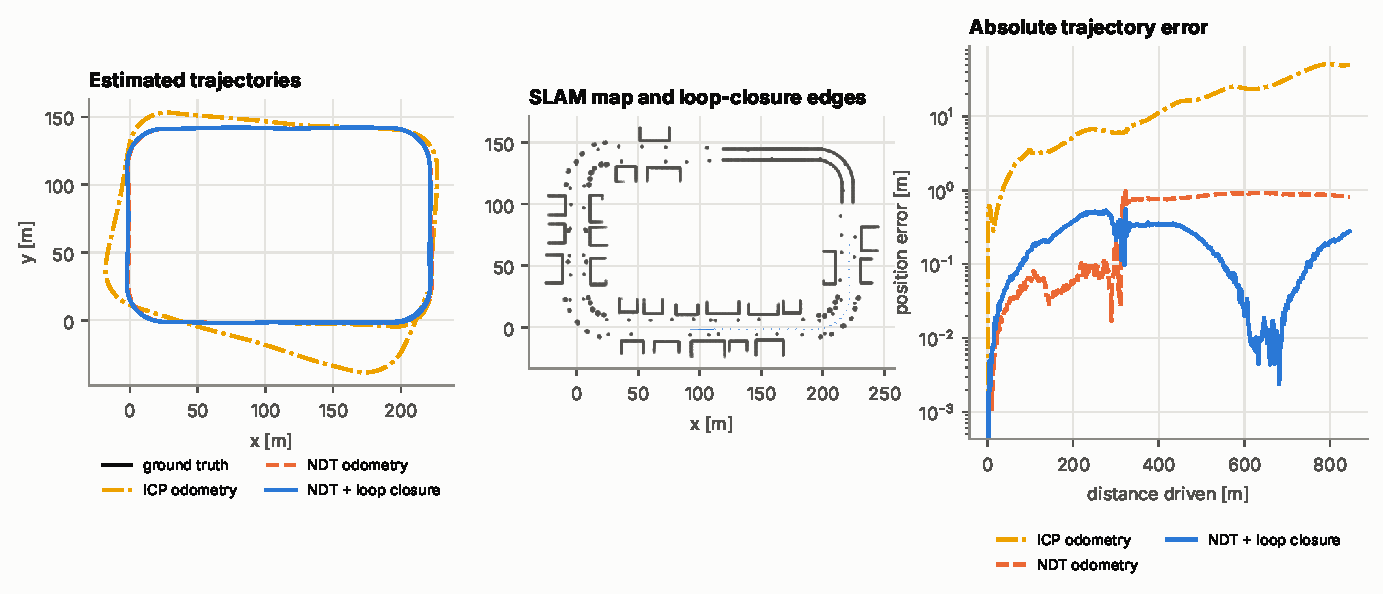
\includegraphics[width=\linewidth]{fig_slam_overview.pdf}
\caption{E2, seed 0. Left: trajectories. Centre: SLAM map and loop-closure edges. Right: absolute trajectory error against distance driven (log scale).}\label{fig:slam}\end{figure}
% AUTO-GENERATED by make_tables.py
\begin{table}[H]\centering\small
\caption{E2: LiDAR SLAM, 1.25 laps, 3 seeds (mean$\pm$std). Map error = distance of map points to noise-free scene geometry [m].}\label{tab:slam}
\begin{adjustbox}{max width=\linewidth}
\begin{tabular}{lrrrrrr}\toprule
Method & ATE RMSE [m] & ATE max [m] & Final [m] & Map mean / P95 [m] & ms/scan & Loops \\ \midrule
ICP odometry (scan-to-scan) & 28.22$\pm$4.61 & 53.17$\pm$2.05 & 52.13$\pm$2.44 & -- & -- & -- \\
NDT scan-to-submap odometry & 0.46$\pm$0.27 & 0.72$\pm$0.37 & 0.52$\pm$0.28 & 0.249 / 0.634 & 14.8 & 0 \\
NDT + loop closure (pose graph) & 0.15$\pm$0.10 & 0.35$\pm$0.19 & 0.14$\pm$0.12 & 0.077 / 0.227 & 30.1 & 32 \\
\bottomrule\end{tabular}\end{adjustbox}
\end{table}

Scan-to-scan ICP drifts to \slamIcp\,m ATE RMSE (final heading error $\approx\slamIcpYaw^\circ$); NDT scan-to-submap odometry reaches \slamNdt\,m; adding loop closure gives \slamLoop\,m with \slamLoops\ loops closed and lowers the mean map error from \slamMapOdom\ to \slamMapLoop\,m (Table~\ref{tab:slam}). In the representative run (Fig.~\ref{fig:slam}, right) the NDT-odometry error steps from $\approx0.1$\,m to $\approx0.8$\,m around the tunnel exit and then stays roughly constant until loop closure removes it. The median NDT Hessian ratio $\rho$ is \slamDegTun\ in the tunnel and \slamDegOut\ elsewhere (\slamDegRatio$\times$ lower; Fig.~\ref{fig:deg}), which is consistent with weak longitudinal constraint in a featureless corridor; the causal link was not isolated (P2).
\textbf{ICP caveat:} in interactive diagnostics (not stored in \texttt{results/}) the per-scan ICP error was small and not tunnel-specific (RMS 4.4\,cm in the tunnel, 2.8\,cm elsewhere), with a mean heading bias of about $-5\times10^{-4}$\,rad per scan in corners that accumulates into the heading drift above. The ICP baseline is untuned (360-beam 2-D scans, $\approx$217 points), so the result says little about ICP in general. The loop count is identical across seeds because the route geometry is identical.
\begin{figure}[H]\centering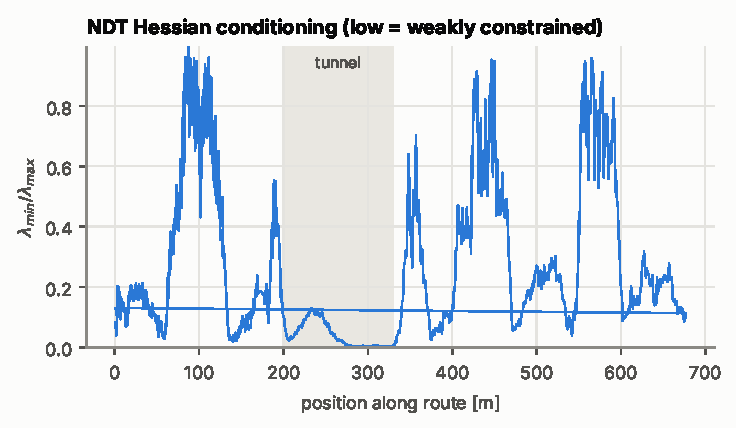
\includegraphics[width=0.6\linewidth]{fig_slam_degeneracy.pdf}\caption{E2: NDT Hessian conditioning along the route (seed 0); lower means weaker constraint.}\label{fig:deg}\end{figure}

\subsection{E3: HD-map localization}
\begin{figure}[H]\centering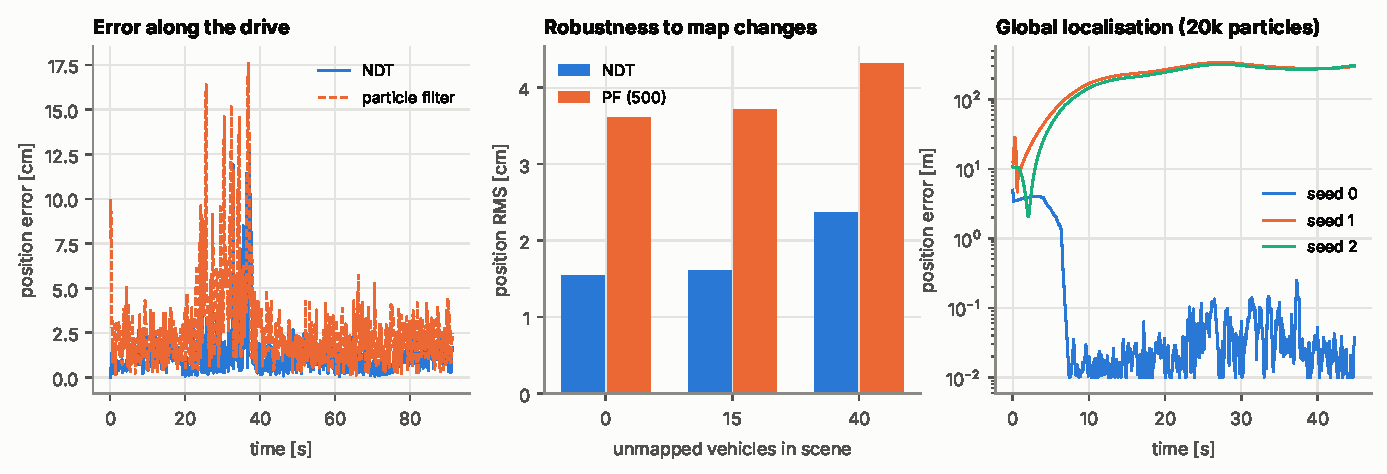
\includegraphics[width=\linewidth]{fig_hdmap_overview.pdf}
\caption{E3. Left: error along the drive (seed 0, 15 unmapped vehicles). Centre: position RMS vs.\ number of unmapped vehicles. Right: global localization from a uniform prior.}\label{fig:hd}\end{figure}
% AUTO-GENERATED by make_tables.py
\begin{table}[H]\centering\small
\caption{E3: localisation against the HD map (3 seeds; mean). Errors in the vehicle frame [cm]; ``unmapped'' = vehicles absent from the map.}\label{tab:hd}
\begin{adjustbox}{max width=\linewidth}
\begin{tabular}{llrrrrrr}\toprule
Unmapped & Method & Lon RMS & Lat RMS & Yaw RMS [deg] & P95 & Max & ms/scan \\ \midrule
0 & NDT & 1.3 & 0.7 & 0.016 & 2.6 & 12.1 & 11.9 \\
 & PF (500) & 3.3 & 1.5 & 0.063 & 7.7 & 19.2 & 1.7 \\
 & VO dead reckoning & 454.0 & 320.9 & 2.636 & 1010.5 & 1079.4 & -- \\
15 & NDT & 1.4 & 0.8 & 0.018 & 2.7 & 12.5 & 11.7 \\
 & PF (500) & 3.4 & 1.6 & 0.068 & 7.7 & 18.5 & 1.6 \\
 & VO dead reckoning & 454.0 & 320.9 & 2.636 & 1010.5 & 1079.4 & -- \\
40 & NDT & 1.9 & 1.4 & 0.044 & 2.8 & 45.2 & 11.5 \\
 & PF (500) & 3.9 & 1.9 & 0.081 & 8.9 & 22.4 & 1.5 \\
 & VO dead reckoning & 454.0 & 320.9 & 2.636 & 1010.5 & 1079.4 & -- \\
\bottomrule\end{tabular}\end{adjustbox}
\end{table}

With 15 unmapped vehicles NDT reaches \hdNdtLon\,cm longitudinal and \hdNdtLat\,cm lateral RMS (max \hdNdtMax\,cm), the particle filter \hdPfLon\,/\,\hdPfLat\,cm; dead reckoning on VO alone is metres off (Table~\ref{tab:hd}). Both degrade gradually as more vehicles are absent from the map, and both peak while driving through the tunnel (Fig.~\ref{fig:hd}, left, $t\approx23$--$38$\,s). The PF error saturates beyond about 1\,000 particles (Table~\ref{tab:pf}). \textbf{Global localization is not reliable:} only \hdGlobOk\ of 3 seeds converged from the uniform prior (Table~\ref{tab:glob}); the other two settled roughly 300\,m from the true pose in this repetitive road geometry.
% AUTO-GENERATED by make_tables.py
\begin{table}[H]\centering\small
\caption{E3: particle-count sweep (seed 0, 15 unmapped vehicles).}\label{tab:pf}
\begin{adjustbox}{max width=\linewidth}
\begin{tabular}{lrrr}\toprule
Particles & Lon RMS [cm] & Lat RMS [cm] & ms/scan \\ \midrule
50 & 4.0 & 2.1 & 0.3 \\
200 & 3.4 & 1.7 & 0.6 \\
1000 & 3.2 & 1.6 & 2.7 \\
3000 & 3.1 & 1.6 & 8.2 \\
\bottomrule\end{tabular}\end{adjustbox}
\end{table}

% AUTO-GENERATED by make_tables.py
\begin{table}[H]\centering\small
\caption{E3: global localisation from a uniform prior (20\,000 particles, 45\,s).}\label{tab:glob}
\begin{adjustbox}{max width=\linewidth}
\begin{tabular}{lrr}\toprule
Seed & Converged at [s] & Final error [m] \\ \midrule
0 & 6.6 & 0.04 \\
1 & not converged & 297.30 \\
2 & not converged & 308.21 \\
\bottomrule\end{tabular}\end{adjustbox}
\end{table}


\subsection{E4: Behaviour tree vs.\ finite-state machine}
% AUTO-GENERATED by make_tables.py
\begin{table}[H]\centering\small
\caption{E4: 300 randomised scenarios (lead vehicle, oncoming traffic, roundabout, pedestrian). Success = route completed without collision.}\label{tab:bt}
\begin{adjustbox}{max width=\linewidth}
\begin{tabular}{lrrlrrrr}\toprule
Controller & Success & of which surprise & Collisions & Time [s] & Hard brakes/run & Emerg. & Aborts \\ \midrule
Behaviour tree & 296/300 & 146/150 & lead 2, oncoming 2 & 84.4 & 1.00 & 7 & 20 \\
FSM-basic (nominal transitions) & 142/300 & 67/150 & roundabout 147, lead 11 & 78.6 & 0.53 & 22 & 0 \\
FSM-full (all pre-emption edges) & 298/300 & 148/150 & oncoming 2 & 86.6 & 0.97 & 7 & 20 \\
FSM-full, re-check edge removed & 149/300 & 74/150 & roundabout 149, oncoming 2 & 79.6 & 0.54 & 7 & 22 \\
\bottomrule\end{tabular}\end{adjustbox}
\par\vspace{2pt}{\footnotesize Surprise = an oncoming vehicle outside the 90\,m perception range appears mid-overtake (150 of 300 scenarios).}
\end{table}

% AUTO-GENERATED by make_tables.py
\begin{table}[H]\centering\small
\caption{E4: structural size of the decision logic.}\label{tab:struct}
\begin{adjustbox}{max width=\linewidth}
\begin{tabular}{lrrr}\toprule
Quantity & BT & FSM (nominal) & FSM (full) \\ \midrule
Nodes / states & 26 & 10 & 10 \\
Transitions & -- & 24 & 38 \\
Edits to add one global-priority behaviour & 3 nodes & -- & 11 transitions \\
\bottomrule\end{tabular}\end{adjustbox}
\end{table}

\begin{figure}[H]\centering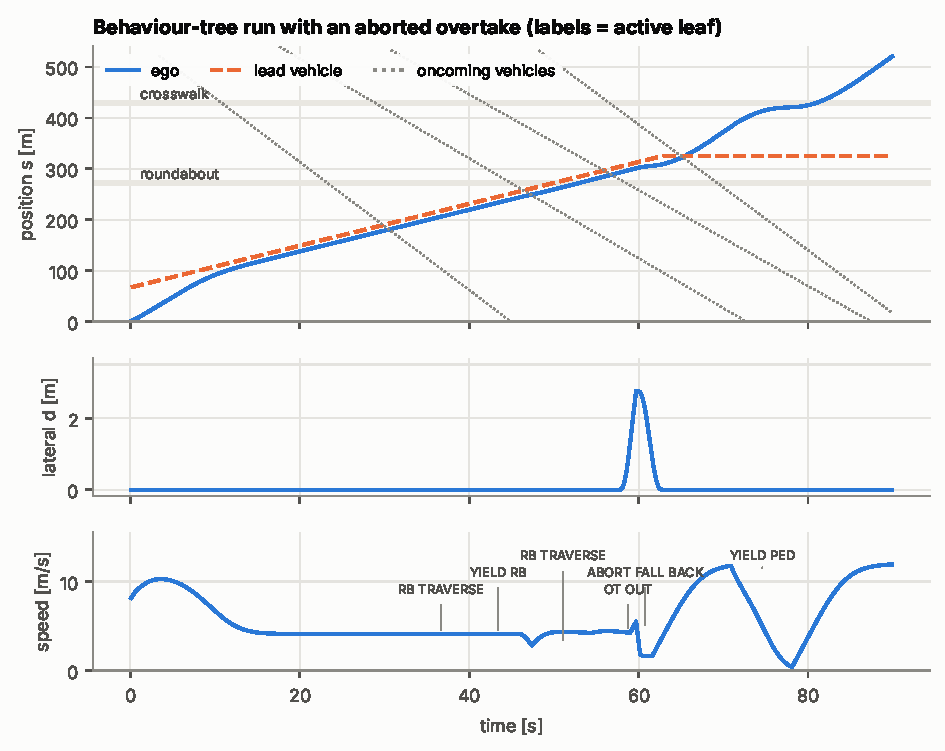
\includegraphics[width=0.78\linewidth]{fig_bt_timeline.pdf}
\caption{E4: one BT run (labels = active leaf). The ego follows a slow lead through the roundabout (yield, traverse), starts an overtake at about 59\,s, aborts it shortly afterwards (\texttt{ABORT FALL BACK}) as an oncoming vehicle approaches, and later yields at the crosswalk.}\label{fig:timeline}\end{figure}
\begin{figure}[H]\centering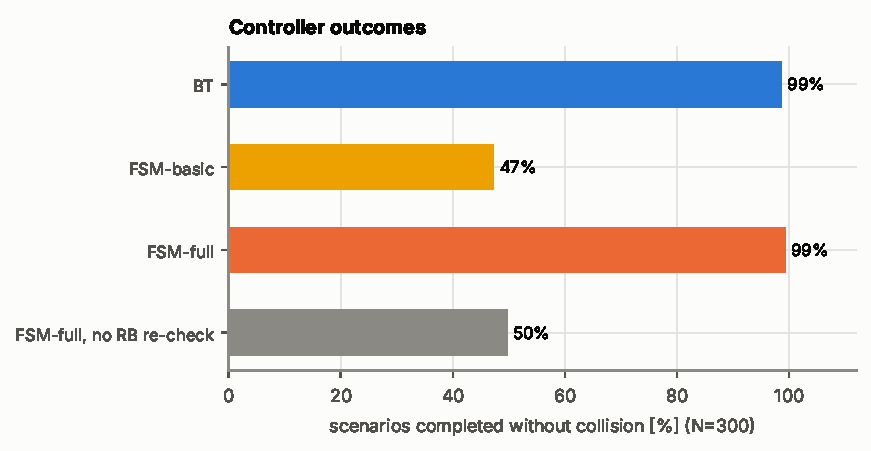
\includegraphics[width=0.55\linewidth]{fig_bt_outcomes.pdf}\caption{E4: share of scenarios completed without collision.}\end{figure}
The BT completes \btOk/300 scenarios, FSM-full \fsmFullOk/300 and FSM-basic \fsmBasicOk/300 (Table~\ref{tab:bt}). FSM-basic fails almost entirely at the roundabout: once the gap check first succeeds (evaluated from 60\,m before the yield line on vehicles expected within a 9\,s window) it switches to the traversal state, which has no edge back to re-check. Removing that single re-check edge from FSM-full gives \fsmNoRecheckOk/300, so the gap is caused by one missing transition, not by FSMs as such; this omission was in my first ``full'' FSM and was found through the collisions. The BT needed no extra wiring because the gap condition is re-evaluated on every tick. \textbf{With all edges added, the FSM is as safe as the BT} (298 vs.\ 296 successes here), so the BT advantage measured is structural: \btNodes\ nodes against \fsmTrans\ transitions, and 3 nodes against 11 transitions to add one global-priority behaviour (Table~\ref{tab:struct}). The BT aborted an overtake in \btAborts\ scenarios. Its 4 failures (2 lead, 2 oncoming) are not yet root-caused (P2).

\subsection{E5: Motion planning}
\begin{figure}[H]\centering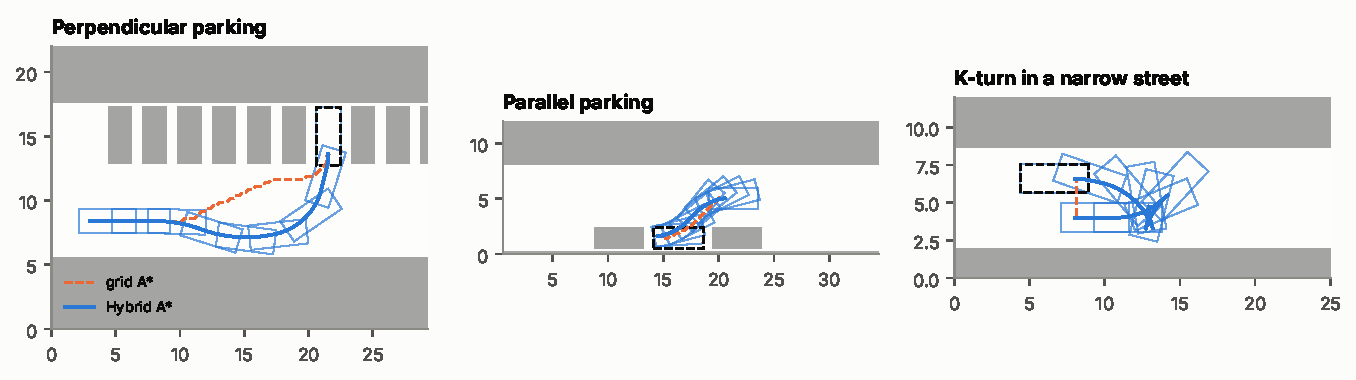
\includegraphics[width=\linewidth]{fig_parking.pdf}
\caption{E5: Hybrid A* (blue, footprints every few poses; dashed black = goal pose) and grid A* (orange) from the nominal start poses.}\label{fig:park}\end{figure}
% AUTO-GENERATED by make_tables.py
\begin{table}[H]\centering\small
\caption{E5: tight-space planning, 6 start poses per scenario. Feasible = collision-free (exact footprint), curvature $\le$ 0.212\,m$^{-1}$, goal pose reached. Means over found paths.}\label{tab:park}
\begin{adjustbox}{max width=\linewidth}
\begin{tabular}{llrrrrrr}\toprule
Scenario & Planner & Feasible & Time [s] & Cusps & Max $|\kappa|$ [1/m] & Collision frac. & Goal head. err [deg] \\ \midrule
Perpendicular parking & Hybrid A* & 6/6 & 0.9 & 0.0 & 0.21 & 0 & $<$6 \\
 & Grid A* & 0/6 & -- & -- & 2.60 & 0.21 & 45 \\
 & Grid A* + Chaikin & 0/6 & -- & -- & 3.96 & 0.23 & 45 \\
Parallel parking & Hybrid A* & 4/6 & 13.7 & 3.0 & 0.21 & 0 & $<$6 \\
 & Grid A* & 0/6 & -- & -- & 2.17 & 0.66 & 172 \\
 & Grid A* + Chaikin & 0/6 & -- & -- & 3.30 & 0.67 & 172 \\
K-turn in a narrow street & Hybrid A* & 6/6 & 9.3 & 4.0 & 0.21 & 0 & $<$6 \\
 & Grid A* & 0/6 & -- & -- & 1.74 & 0.57 & 98 \\
 & Grid A* + Chaikin & 0/6 & -- & -- & 2.64 & 0.58 & 98 \\
\bottomrule\end{tabular}\end{adjustbox}
\end{table}

Hybrid A* found a feasible path in \hyPerp\ (perpendicular), \hyPar\ (parallel) and \hyK\ (K-turn) trials. In parallel parking 2 of 6 starts were not solved within the 40\,s / 60\,000-expansion budget; solved cases took \hyParTime\,s on average (pure Python, not real-time) and ended about \hyParErr\,cm from the nominal goal (accepted tolerance 30\,cm, 5$^\circ$; an exact Dubins connection is used when one exists). Grid A* produced paths in every trial but none was feasible: curvature of 1.7--4.0\,m$^{-1}$ against the 0.212\,m$^{-1}$ limit, 21--67\% of poses colliding when checked with the true footprint, and goal-heading errors of 45--172$^\circ$. This baseline has no heading in its state, so these failures are expected by construction; the comparison shows what the extra state buys.
\begin{figure}[H]\centering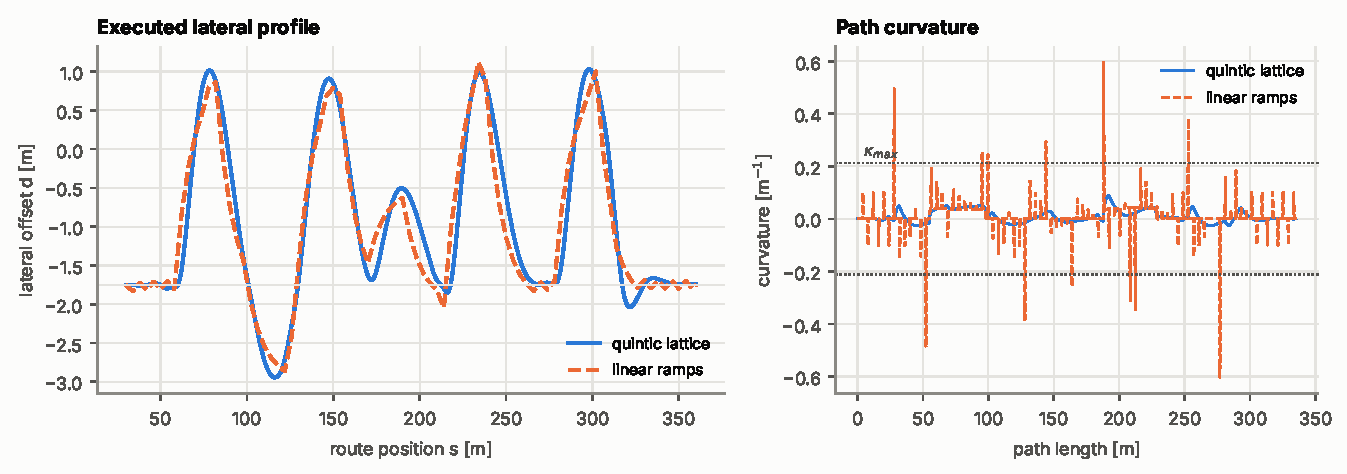
\includegraphics[width=\linewidth]{fig_lattice.pdf}
\caption{E5: executed lateral profile and curvature on the route with 7 obstacles (5 vehicles, 2 small objects); dotted = vehicle curvature limit.}\label{fig:lat}\end{figure}
% AUTO-GENERATED by make_tables.py
\begin{table}[H]\centering\small
\caption{E5: receding-horizon lateral planning on 20 random obstacle layouts. OK = collision-free and curvature within the vehicle limit.}\label{tab:lat}
\begin{adjustbox}{max width=\linewidth}
\begin{tabular}{lrrrrr}\toprule
Profile & OK & Collision-free & Max $|\kappa|$ [1/m] & Max $|d\kappa/dl|$ [1/m$^2$] & Replans w/o candidate \\ \midrule
quintic & 16/20 & 16/20 & 0.075$\pm$0.015 & 0.07$\pm$0.00 & 45 \\
linear & 0/20 & 16/20 & 0.674$\pm$0.251 & 2.61$\pm$0.97 & 66 \\
\bottomrule\end{tabular}\end{adjustbox}
\par\vspace{2pt}{\footnotesize Curvature rate depends on the 0.25\,m sampling of the executed path for the kinked baseline.}
\end{table}

Both lateral profiles use the same candidates and collision test and are collision-free in the same layouts, but only the quintic lattice stays within the curvature limit: \latQuinticOk\ OK layouts against \latLinearOk, peak curvature \latQuinticK\ vs.\ \latLinearK\,m$^{-1}$ (limit \kappaMax; Fig.~\ref{fig:lat}). In the 4 layouts that fail for both, some replans had no feasible candidate; whether those layouts admit any collision-free path was not checked (P7).

\subsection{E6: Hybrid A* slot length and search speed}
\begin{figure}[H]\centering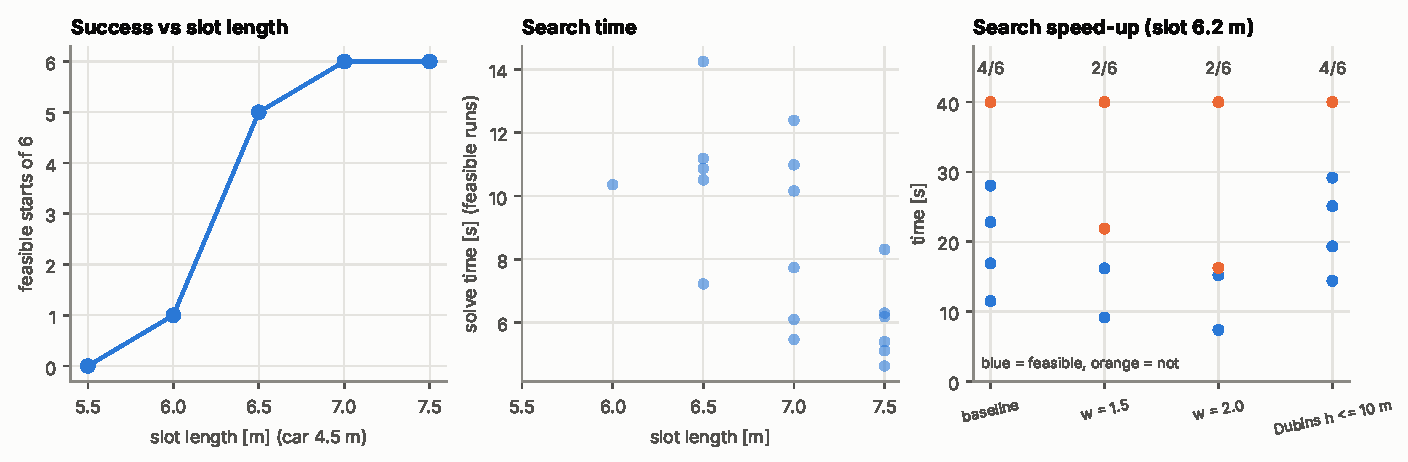
\includegraphics[width=\linewidth]{fig_hybrid_sweep.pdf}
\caption{E6. Left: feasible starts vs.\ slot length. Centre: solve time of feasible runs. Right: search variants on the 6.2\,m slot (run time capped at 40\,s).}\label{fig:hysweep}\end{figure}
% AUTO-GENERATED by make_tables.py
\begin{table}[H]\centering\small
\caption{E6: Hybrid A* parallel parking vs.\ slot length (car 4.5\,m, 6 start poses per slot, 40\,s / 60\,000-expansion budget). Time, expansions, cusps and length are means over feasible runs.}\label{tab:slot}
\begin{adjustbox}{max width=\linewidth}
\begin{tabular}{rrrrrr}\toprule
Slot [m] & Feasible & Median time [s] & Expansions & Cusps & Length [m] \\ \midrule
5.5 & 0/6 & -- & -- & -- & -- \\
6.0 & 1/6 & 10.4 & 12372 & 2.0 & 8.4 \\
6.5 & 5/6 & 10.9 & 12637 & 3.4 & 10.6 \\
7.0 & 6/6 & 8.9 & 8743 & 2.2 & 10.0 \\
7.5 & 6/6 & 5.8 & 6836 & 2.0 & 10.3 \\
\bottomrule\end{tabular}\end{adjustbox}
\end{table}

% AUTO-GENERATED by make_tables.py
\begin{table}[H]\centering\small
\caption{E6: search-speed variants on the nominal 6.2\,m slot (same 6 start poses, run back to back on the same machine).}\label{tab:speed}
\begin{adjustbox}{max width=\linewidth}
\begin{tabular}{lrrrr}\toprule
Variant & Feasible & Median time [s] & Expansions & Length [m] \\ \midrule
Baseline ($w=1$) & 4/6 & 19.8 & 14376 & 9.6 \\
Weighted A*, $w=1.5$ & 2/6 & 12.7 & 8520 & 8.9 \\
Weighted A*, $w=2$ & 2/6 & 11.3 & 7504 & 9.1 \\
Dubins term only within 10\,m & 4/6 & 22.2 & 17949 & 9.4 \\
\bottomrule\end{tabular}\end{adjustbox}
\end{table}

Feasible starts are \slotOkA, \slotOkB, \slotOkC, \slotOkD\ and \slotOkE\ for slots of 5.5, 6.0, 6.5, 7.0 and 7.5\,m (Table~\ref{tab:slot}), and solve time falls as the slot widens. The threshold, between 6.0 and 7.0\,m for a 4.5\,m car, belongs to this planner (primitive set, $0.5$\,m/$5^\circ$ grid, 8\,cm margin, 40\,s/60\,000-expansion budget); whether the 5.5--6.0\,m failures are geometric limits or budget limits was not tested.
Weighted A* ($w=1.5$ and $2$) removes about 40--50\% of the expansions and lowers the median time from \spdBaseTime\ to \spdWaTime\ and \spdWbTime\,s, but solves only \spdWaOk\ and \spdWbOk\ starts against \spdBaseOk\ (Table~\ref{tab:speed}). Restricting the Dubins heuristic term to 10\,m made the search \emph{slower} (\spdDubExp\ against \spdBaseExp\ expansions) at equal success. \textbf{No variant gave a speed-up without losing solutions}; the compiled port (P5) is still open. Wall-clock times vary between runs on this shared machine (an earlier run gave a 12\,s median for the same, deterministic baseline searches), so expansions are the reliable comparison.

\subsection{E7: lattice failure analysis}
\begin{figure}[H]\centering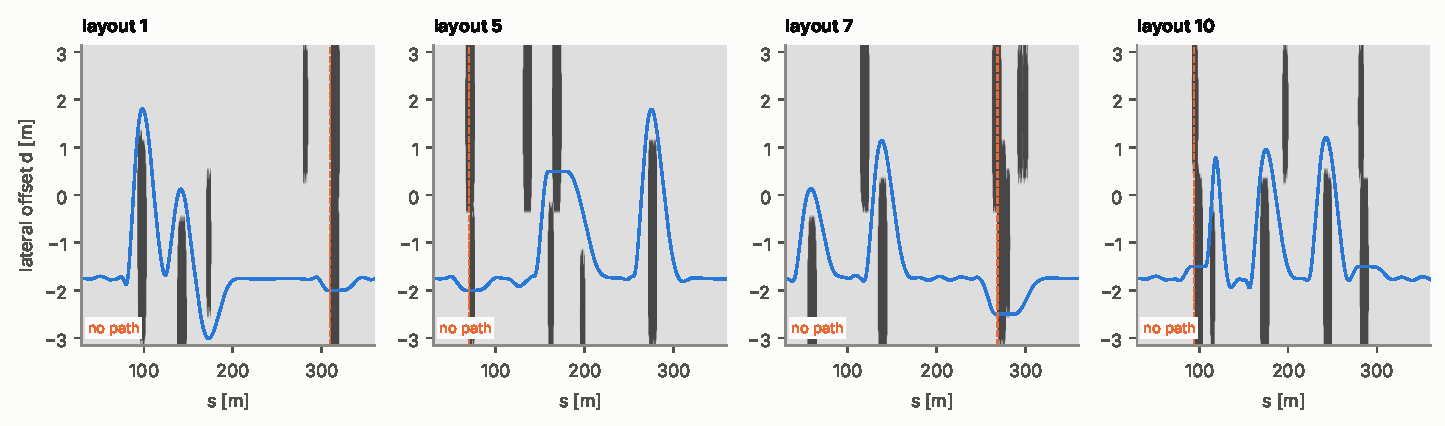
\includegraphics[width=\linewidth]{fig_lattice_failures.pdf}
\caption{E7: the layouts in which the quintic lattice fails. Dark = cells blocked for the 3-disc body at road heading, light = free; blue = executed path; dashed orange = first collision.}\label{fig:latfail}\end{figure}
% AUTO-GENERATED by make_tables.py
\begin{table}[H]\centering\small
\caption{E7: the layouts in which the quintic lattice fails. ``Corridor path'' = a Frenet-grid search finds any path from the start to $s=360$\,m inside the 6.2\,m corridor (lateral slope $\le0.4$, 3-disc body at road heading), with zero clearance and with the planner's 0.35\,m margin; the last three columns re-run the planner with a denser lattice, 2\,m replanning, or both.}\label{tab:latfail}
\begin{adjustbox}{max width=\linewidth}
\begin{tabular}{rrccccc}\toprule
Layout & Obstacles & Corridor path, 0\,m & Corridor path, 0.35\,m & Dense & 2\,m replan & Both \\ \midrule
1 & 14 & no & no & no & no & no \\
5 & 15 & no & no & no & no & no \\
7 & 18 & no & no & no & no & no \\
10 & 16 & no & no & no & no & no \\
\bottomrule\end{tabular}\end{adjustbox}
\end{table}

In \lfSolvZero\ of the \lfFail\ failing layouts a Frenet-grid search finds any path inside the corridor, even with zero clearance, and a denser lattice (25 offsets, five horizons), 2\,m replanning or both recover \lfRecovered\ of them (Table~\ref{tab:latfail}). Fig.~\ref{fig:latfail} shows why: each contains a column of obstacles covering the whole 6.2\,m corridor. Under the stated assumptions these are infeasible layouts, not planner faults, which supports the P7 hypothesis for this set. \textbf{Caveats:} the search is approximate (road-heading body, lateral slope $\le0.4$, corridor limits); with the planner's 0.35\,m margin it also marks \lfOkUnsolv\ of the 16 passing layouts as unsolvable, because the planner's fallback (keep the previous plan) can pass with less margin; and a wider corridor (oncoming lane) would change the answer.

\subsection{E8: 20-seed statistics and LiDAR degradation}
\begin{figure}[H]\centering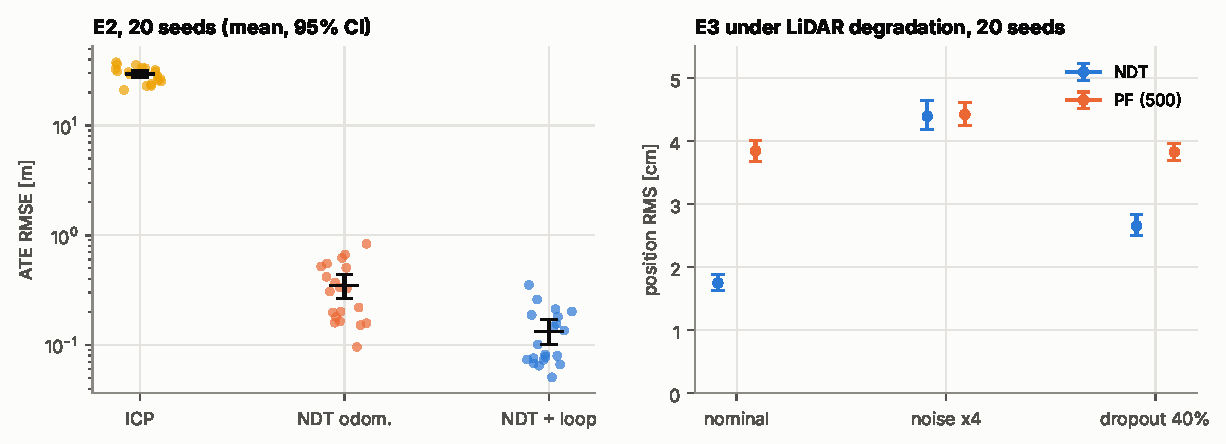
\includegraphics[width=\linewidth]{fig_sensitivity.pdf}
\caption{E8. Left: SLAM ATE RMSE per seed (dots) with mean and 95\% bootstrap CI. Right: HD-map position RMS under LiDAR degradation, mean and 95\% CI.}\label{fig:sens}\end{figure}
% AUTO-GENERATED by make_tables.py
\begin{table}[H]\centering\small
\caption{E8: SLAM ATE RMSE [m] over 20 seeds: mean with 95\% bootstrap CI of the mean, median and standard deviation.}\label{tab:sens_slam}
\begin{adjustbox}{max width=\linewidth}
\begin{tabular}{lrrr}\toprule
Method & Mean [95\% CI] & Median & Std \\ \midrule
ICP odometry & 29.4 [27.4, 31.4] & 30.14 & 4.78 \\
NDT odometry & 0.35 [0.26, 0.44] & 0.32 & 0.21 \\
NDT + loop closure & 0.13 [0.10, 0.17] & 0.09 & 0.08 \\
\bottomrule\end{tabular}\end{adjustbox}
\end{table}

% AUTO-GENERATED by make_tables.py
\begin{table}[H]\centering\small
\caption{E8: HD-map localization under LiDAR degradation (20 seeds, 15 unmapped vehicles). Position RMS [cm], mean with 95\% bootstrap CI; ``fail'' = maximum error above 1\,m.}\label{tab:sens_loc}
\begin{adjustbox}{max width=\linewidth}
\begin{tabular}{lrrrr}\toprule
LiDAR & NDT RMS [cm] & NDT fail & PF RMS [cm] & PF fail \\ \midrule
nominal & 1.7 [1.6, 1.9] & 0/20 & 3.8 [3.7, 4.0] & 0/20 \\
noise $\times$4 & 4.4 [4.2, 4.6] & 1/20 & 4.4 [4.2, 4.6] & 0/20 \\
dropout 40\% & 2.7 [2.5, 2.8] & 0/20 & 3.8 [3.7, 4.0] & 0/20 \\
\bottomrule\end{tabular}\end{adjustbox}
\end{table}

With \sensSeeds\ seeds the SLAM ATE (mean [95\% CI], m) is \sensSlamIcp\ for ICP, \sensSlamOdom\ for NDT odometry and \sensSlamLoop\ with loop closure; the intervals do not overlap, so the ordering of E2 holds. The 3-seed means of E2 were slightly higher for NDT odometry (0.46\,m) than the 20-seed mean. For HD-map localization (15 unmapped vehicles) the nominal position RMS is \sensNdtNom\,cm for NDT and \sensPfNom\,cm for the particle filter. Four times the LiDAR noise raises NDT to \sensNdtNoise\,cm (\sensNdtNoiseFail\ runs with a maximum error above 1\,m) and the PF to \sensPfNoise\,cm; 40\% dropout gives \sensNdtDrop\ and \sensPfDrop\,cm. NDT is the more sensitive of the two and loses its accuracy advantage at $4\times$ noise; the PF is nearly insensitive but never better than NDT. Only LiDAR noise and dropout were varied; VO/IMU noise (partly covered in E1) and map age remain open (P3).

\subsection{E9: closed-loop integration}
\begin{figure}[H]\centering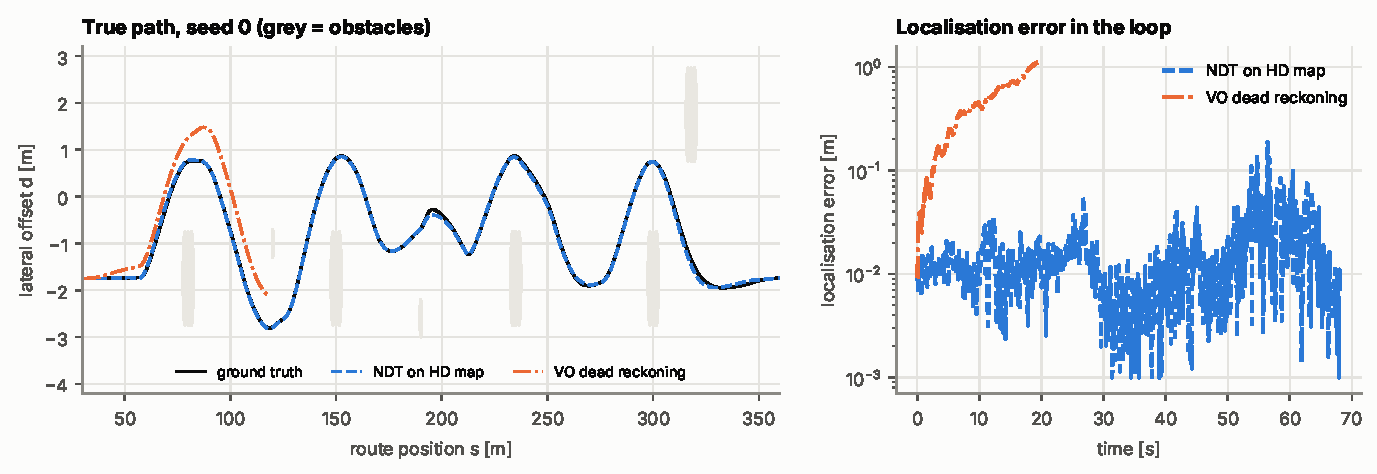
\includegraphics[width=\linewidth]{fig_closed_loop.pdf}
\caption{E9, seed 0. Left: true path in Frenet coordinates for the three pose sources (grey = obstacles, stretched by the unequal axes). Right: localization error in the loop.}\label{fig:cl}\end{figure}
% AUTO-GENERATED by make_tables.py
\begin{table}[H]\centering\small
\caption{E9: closed loop (pose source $\to$ behaviour tree $\to$ lattice $\to$ pure pursuit $\to$ bicycle model), 10 runs per pose source, 7 obstacles on a 330\,m route. Clearance is the minimum body-to-obstacle gap; cross-track is the distance of the true position to the current plan.}\label{tab:cl}
\begin{adjustbox}{max width=\linewidth}
\begin{tabular}{lrrrrrr}\toprule
Pose source & Success & Collisions & Min clearance [m] & Loc. RMS [cm] & Cross-track RMS [m] & Replans w/o candidate \\ \midrule
Ground-truth pose & 10/10 & 0 & 0.50$\pm$0.00 & 0.0$\pm$0.0 & 0.16$\pm$0.00 & 7.0$\pm$0.0 \\
NDT on HD map & 10/10 & 0 & 0.48$\pm$0.02 & 3.1$\pm$0.7 & 0.15$\pm$0.00 & 5.5$\pm$1.7 \\
VO dead reckoning & 0/10 & 10 & -0.08$\pm$0.05 & 61.5$\pm$30.6 & 0.52$\pm$0.25 & 1.5$\pm$1.5 \\
\bottomrule\end{tabular}\end{adjustbox}
\end{table}

With ground-truth pose the stack completes \clGt\ runs. NDT on the HD map matches it (\clNdt) at \clNdtLoc\,cm RMS localization error, with essentially the same cross-track error (\clCte\,m RMS) and nearly the same clearance (\clClrNdt\ vs.\ \clClrGt\,m): at this accuracy localization is not the limiting factor, the tracker is. VO dead reckoning succeeds in \clDr: its error reaches about 1\,m (RMS \clDrLoc\,m) before the first obstacle and every run ends in a collision (Fig.~\ref{fig:cl}), consistent with the P4 hypothesis. \textbf{Caveats:} perfect obstacle perception, one layout and route, simulated VO, a kinematic plant without tyre slip or actuator delay, a three-behaviour BT, and no VIO EKF in the loop (the E1 filter runs offline); the dead-reckoning baseline stands in for a VIO outage and is not the E1 filter.

\section{Discussion}
\textbf{Two accuracy layers.} VIO keeps the vehicle within about a metre through a 130\,m outage (E1), whereas map-based localization reaches centimetres (E3). The first provides \emph{continuity} when external references are missing, the second \emph{accuracy} when a map is available; in a full stack the VIO output is the prior that NDT or the particle filter refines. The tunnel is the hard case for every module, for different reasons: the dead-reckoning error accumulates (E1; in the simulator VO noise is deliberately inflated there), the NDT Hessian is poorly conditioned (E2), and the map-based error peaks (E3). The Hessian ratio $\rho$ is cheap to compute and could gate or down-weight scan-matching updates in the filter; this was not tested.

\textbf{Loop closure buys consistency, not local accuracy.} NDT odometry is already sub-metre over 846\,m; the pose graph reduces ATE from \slamNdt\ to \slamLoop\,m and, more usefully, removes the step introduced near the tunnel exit, giving a map error of \slamMapLoop\,m. The scan-to-scan ICP baseline, in contrast, is unusable without a map-based correction.

\textbf{BT versus FSM.} The measured difference between a BT and a \emph{complete} FSM is not safety but specification effort. The first FSM-full omitted one edge (roundabout re-check) and lost about half of the scenarios; the BT does not need that edge because every condition is re-evaluated on each tick. Complete FSMs close the gap but need \fsmTrans\ transitions instead of \btNodes\ nodes, and adding a global-priority behaviour costs 11 transitions against 3 nodes. A different FSM designer could narrow or widen this gap, so the claim is about how failure arises (a missing edge) rather than a universal ranking. That the BT still failed 4 of 300 scenarios shows that tree structure alone does not guarantee safety.

\textbf{Feasibility is a property of the state space.} Grid~A* optimizes length over positions only, so it can neither respect $\kappa_{\max}$ nor the footprint; Hybrid~A* pays seconds of search time in Python (and failed on two of six parallel-parking starts within budget) for paths a car can drive. The quintic lattice trades a little lateral agility for a curvature rate about 35 times lower than the linear-ramp baseline ($0.073$ vs.\ $2.6$\,m$^{-2}$ in E5).

\textbf{Error budget (E8, E9).} NDT's centimetre-level error is about an order of magnitude below the planner's 0.35\,m margin and leaves the closed loop unchanged, whereas VO dead reckoning exceeds the margin within tens of metres. The 20-seed intervals show that the method ranking of E2 is not a small-sample artefact, and that NDT, not the particle filter, is the component whose accuracy degrades with LiDAR quality.

\textbf{Negative results.} Neither cheap speed-up of Hybrid~A* (weighted heuristic, shorter Dubins range) improved time-to-solution without losing solutions, and the failing lattice layouts are blocked rather than hard (E6, E7).

\textbf{Implication for integration.} The filter's covariance was conservative (E1) and NDT/PF errors are small relative to lane width, but global localization is the weak link (E3); a deployed system would need place recognition or a GNSS-seeded prior for initialization and recovery.

\section{Real-world applications}
\begin{itemize}
\item \textbf{Tunnels, urban canyons, parking structures:} inertial/visual dead reckoning bridges GNSS gaps (E1); production systems add wheel odometry and map constraints.
\item \textbf{Map-based localization:} point-cloud NDT scan matching against a pre-built map is used in open-source stacks such as Autoware~\cite{kato18}; a particle filter adds multi-hypothesis recovery at the cost of accuracy (E3).
\item \textbf{Map building and updating:} LiDAR SLAM with loop closure is the core of survey-vehicle and fleet mapping pipelines (E2).
\item \textbf{Tactical decision making:} BTs keep priorities explicit and let behaviours be added as subtrees; they are widely used in robotics, e.g.\ in the ROS~2 navigation stack~\cite{macenski20} (E4).
\item \textbf{Automated valet parking, depots, K-turns:} Hybrid~A* free-space planning, as in open-space planners of Apollo~\cite{fan18} and Autoware~\cite{kato18} (E5); Frenet lattices serve on-road lane changes and obstacle nudging.
\end{itemize}

\section{Limitations and threats to validity}\label{sec:limits}
\begin{itemize}
\item \textbf{Simulation only.} 2-D, one synthetic world; no 3-D LiDAR, motion distortion, weather, rolling shutter. The simulator's error models define the results; centimetre figures are not claims about real vehicles.
\item \textbf{VIO is not visual.} No feature tracking or IMU--camera calibration; VO is simulated and the IMU model is planar.
\item \textbf{Optimistic HD map.} Built with near-true poses from the same geometry; the only map change tested is unmapped vehicles; NDT is seeded with simulated VO.
\item \textbf{Baselines.} ICP is untuned; the FSMs are my own designs and the BT--FSM comparison depends on which edges exist; E4 uses point-mass dynamics with perfect tracking.
\item \textbf{Small samples, no significance tests.} E2 and E3 use 3 seeds, E5 parking 6 starts; standard deviations are indicative only.
\item \textbf{Extended experiments.} E6 uses 6 starts per slot and machine-dependent timings; E7's solvability test is approximate; E8 varies only LiDAR noise and dropout; E9 has perfect perception, one layout, a kinematic plant and no VIO filter in the loop.
\item \textbf{Unexplained results.} The 4 BT failures, the NDT step near the tunnel exit, the ICP heading bias and the 4 lattice layouts that fail were not root-caused.
\item \textbf{Speed and integration.} Hybrid~A* takes seconds in Python; the LOAM-style feature extractor is implemented but not evaluated; modules are not integrated in closed loop.
\end{itemize}

\section{Conclusions}
All five objectives were implemented and measured in simulation, followed by four extended experiments.
\textbf{O1:} VIO keeps tunnel-exit error at \vioExitVio\,m (20 seeds), about $2\times$ better than GPS+IMU without vision and over $25\times$ better than the IMU alone.
\textbf{O2:} NDT SLAM with loop closure reaches \slamLoop\,m ATE over 846\,m with a \slamMapLoop\,m mean map error; scan-to-scan ICP does not.
\textbf{O3:} NDT and PF localize to \hdNdtLon--\hdPfLon\,cm (longitudinal RMS) with 15 unmapped vehicles, but global localization succeeded in only \hdGlobOk\ of 3 seeds.
\textbf{O4:} the BT completed \btOk/300 scenarios; a complete FSM \fsmFullOk/300; the BT's advantage is its compact, re-evaluated structure, not higher safety.
\textbf{O5:} Hybrid~A* produced feasible paths in 16 of 18 trials and the quintic lattice in \latQuinticOk\ layouts, while grid-based paths were never feasible.
\textbf{Extended runs:} Hybrid~A* needs a parallel slot of about 6.5--7\,m here (E6) and no tested search shortcut preserves its success rate; the lattice's \lfFail\ failures are blocked layouts (E7); the SLAM and HD-map conclusions hold over \sensSeeds\ seeds (E8); and with NDT localization the full stack completes \clNdt\ closed-loop runs against \clDr\ for dead reckoning (E9).
These conclusions hold for the simulator and parameter choices documented here; the next step is closed-loop integration and validation on real data (Section~\ref{sec:future}).

\section{Future work}\label{sec:future}
\subsection{Planned experiments and status}\label{sec:plan}
\begin{table}[H]\centering\small
\caption{Planned experiments and status. Hypotheses are expectations, not findings; results of the experiments that were run are in the cited sections.}
\begin{tabular}{@{}l>{\raggedright}p{2.2cm}>{\raggedright}p{4.6cm}>{\raggedright}p{3.0cm}>{\raggedright\arraybackslash}p{3.1cm}@{}}\toprule
ID & Topic & Experiment & Hypothesis & Status\\\midrule
P1 & LOAM features & Edge/planar-feature scan-to-map odometry (\texttt{extract\_loam\_features}) vs NDT & Faster per scan, worse in the tunnel & not run\\
P2 & Root causes & Inspect the 4 BT failures; ICP rotation bias vs.\ turn rate; NDT step at tunnel exit & Unknown for BT; ICP bias grows with turn rate & not run\\
P3 & Sensitivity, statistics & LiDAR noise/dropout; VO/IMU noise; map age; 20 seeds with bootstrap CIs & Graceful degradation, then a cliff & partly run (E8): E2/E3, LiDAR noise and dropout\\
P4 & Integration & Pose $\to$ BT $\to$ lattice $\to$ tracker, closed loop & Localization error small against lane margins & partly run (E9): NDT yes, VIO filter not in loop\\
P5 & Hybrid~A* & Slot-length sweep, search speed-up, goal refinement, compiled port & Threshold near the geometric minimum slot & partly run (E6): sweep and heuristic variants; no compiled port\\
P6 & Global localization & More particles, heading prior, place recognition; 20 seeds & Place-recognition seeding fixes most failures & not run\\
P7 & Lattice & Solvability of the 4 failing layouts; speed dimension; moving obstacles & Failures are infeasible layouts & partly run (E7): solvability only\\
P8 & Real data & NDT/SLAM on a public LiDAR odometry dataset (e.g.\ KITTI~\cite{geiger12}) & Same ranking ICP $<$ NDT $<$ NDT+loop & not run\\\bottomrule
\end{tabular}\end{table}

\subsection{Experiment log (extend this table)}
Add one \verb|\logrow| line per run (format as below), then recompile.
\newcommand{\logrow}[5]{#1 & #2 & #3 & #4 & #5 \\}
\begin{table}[H]\centering\footnotesize
\caption{Experiment log.}
\begin{tabular}{llp{2.9cm}p{3.6cm}p{4.2cm}}\toprule
Date & ID & Config / seeds & Key result & Observation\\\midrule
\logrow{Nov 2026}{E1}{20 seeds}{VIO tunnel exit \vioExitVio\,m}{metre-level; VO simulated}
\logrow{Nov 2026}{E2}{3 seeds}{NDT+loop ATE \slamLoop\,m}{ICP drifts; tunnel $\rho$ \slamDegRatio$\times$ lower}
\logrow{Nov 2026}{E3}{3 seeds $\times$ 3 levels}{NDT \hdNdtLon/\hdNdtLat\,cm}{global localization \hdGlobOk/3}
\logrow{Nov 2026}{E4}{300 scenarios}{BT \btOk, FSM-full \fsmFullOk}{one missing edge: \fsmNoRecheckOk}
\logrow{Nov 2026}{E5}{3 maps, 20 layouts}{Hybrid A* \hyPerp, \hyPar, \hyK}{lattice \latQuinticOk\ vs linear \latLinearOk}
\logrow{Nov 2026}{E6}{5 slots $\times$ 6 starts; 4 variants}{feasible \slotOkA/\slotOkB/\slotOkC/\slotOkD/\slotOkE}{no speed-up without loss}
\logrow{Nov 2026}{E7}{20 layouts, 4 failing}{\lfSolvZero\ of \lfFail\ solvable}{blocked corridors}
\logrow{Nov 2026}{E8}{\sensSeeds\ seeds; 3 LiDAR settings}{NDT+loop \sensSlamLoop\,m}{ranking holds; NDT sensitive to noise}
\logrow{Nov 2026}{E9}{3 pose sources $\times$ 10}{NDT \clNdt, VO \clDr}{localization not limiting at 3\,cm}
% add new rows above this line
\bottomrule\end{tabular}\end{table}

\subsection{Research ideas beyond this week}
\textbf{Estimation and mapping}
\begin{enumerate}[series=ideas,label=\textbf{I\arabic*.},leftmargin=2.4em]
\item \textbf{Real visual front end:} KLT/ORB tracking with an MSCKF or sliding-window back end and IMU preintegration~\cite{mourikis07,forster17}; validate on EuRoC~\cite{burri16}.
\item \textbf{Tightly coupled LiDAR-inertial odometry} with IMU de-skewing (LIO-SAM/FAST-LIO2 style~\cite{shan20,xu22}) and 3-D LOAM features~\cite{zhang14}.
\item \textbf{Degeneracy-aware fusion:} feed $\rho$ or the Hessian eigenvectors into the EKF covariance, constrain only the well-observed directions~\cite{zhang16}.
\item \textbf{Online calibration:} IMU--camera extrinsics and time offset; observability analysis for planar vehicle motion; wheel odometry and non-holonomic constraints.
\item \textbf{Robust loop closure:} Scan Context place recognition~\cite{kim18}, switchable constraints or max-mixtures~\cite{sunderhauf12}, injected false-loop tests.
\item \textbf{Consistency analysis:} NEES/NIS tests for the EKF, covariance recovery from the pose graph.
\item \textbf{Map maintenance:} change detection, long-term map updating, Lanelet2/OpenDRIVE export~\cite{poggenhans18}.
\item \textbf{Global localization and recovery:} multi-hypothesis NDT, GNSS-seeded priors, kidnapped-robot tests; integrity monitoring and protection levels.
\end{enumerate}
\textbf{Decision making}
\begin{enumerate}[resume*=ideas]
\item \textbf{Closed-loop BT in CARLA}~\cite{dosovitskiy17} or ROS~2 with OpenSCENARIO scenarios; compare BT, hierarchical FSM and a learned policy; scenario coverage metrics.
\item \textbf{Formal verification} of BTs (model checking, runtime monitors) to turn the observed ``missing edge'' failure into a checkable property.
\item \textbf{Behaviour planning under uncertainty:} POMDP or multi-policy planning at the leaf level; learned condition nodes with calibrated confidence.
\end{enumerate}
\textbf{Motion planning and control}
\begin{enumerate}[resume*=ideas]
\item \textbf{Hybrid~A* acceleration:} compiled implementation, Reeds--Shepp expansions~\cite{reeds90}, learned or lookup heuristics, anytime search.
\item \textbf{Trajectory refinement:} optimization-based smoothing and collision avoidance~\cite{zhang21} on top of the Hybrid~A* path; slot-length sweep for parallel parking.
\item \textbf{Space-time lattice:} speed and time dimension, moving obstacles, jerk limits, comparison with RRT* and optimization-based planners.
\item \textbf{Tracking control:} pure pursuit/Stanley/MPC on a dynamic bicycle model with tyre slip, closed-loop with the planners.
\end{enumerate}
\textbf{System and validation}
\begin{enumerate}[resume*=ideas]
\item \textbf{Closed-loop integration} of all modules with latency budget and fault injection (sensor dropout, delayed GPS, map mismatch).
\item \textbf{Public data:} KITTI~\cite{geiger12}, nuScenes~\cite{caesar20}, Newer College or Oxford RobotCar for SLAM/localization; ATE/RPE protocol~\cite{zhang18}.
\item \textbf{Statistical protocol:} more seeds, bootstrap confidence intervals, paired comparisons, pre-registered hypotheses.
\item \textbf{Embedded deployment:} real-time profiling on an automotive-class computer; C++/ROS~2 port of the modules that exceed their time budget.
\item \textbf{Safety argument:} SOTIF-style hazard analysis for the failure modes found here (global-localization failure, missed roundabout re-check, unsolved parking).
\end{enumerate}

\section{Reproducibility and folder structure}\label{sec:repro}
\noindent\begin{minipage}{\linewidth}\begin{lstlisting}[basicstyle=\ttfamily\footnotesize,frame=single]
sdc_project/
|-- main.tex, main.pdf        this report (pdfLaTeX, run twice)
|-- numbers.tex, tables/      generated by make_tables.py from results/*.json
|-- make_tables.py, run_all.py, requirements.txt, README.md
|-- FUTURE_IDEAS.md          research ideas (same list as Sec. Future work)
|-- sdc/                      library
|   |-- geometry.py
|   |-- sim/            world.py, drive.py
|   |-- localization/   vio.py, ndt.py, icp.py, pose_graph.py, lidar_slam.py,
|   |                   hd_map.py, particle_filter.py
|   |-- behavior/       bt.py, scenario.py
|   `-- planning/       dubins.py, hybrid_astar.py, scenarios.py, lattice.py
|-- experiments/              common.py, exp1_vio.py ... exp9_closed_loop.py
|-- tests/                    test_core.py (6 unit tests)
`-- results/                  exp*.json (raw numbers), figures/*.pdf|png
\end{lstlisting}\end{minipage}\par\smallskip
\begin{lstlisting}[basicstyle=\ttfamily\footnotesize,frame=single]
pip install -r requirements.txt     # numpy, scipy, matplotlib, pytest
python run_all.py                   # unit tests, E1-E9, tables
python make_tables.py               # after re-running any single experiment
pdflatex main.tex && pdflatex main.tex
\end{lstlisting}
All experiments use fixed seeds; run time depends on the CPU and the number of cores (the experiment scripts use two worker processes). Figures are regenerated into \texttt{results/figures/}; the report reads numbers only through \texttt{numbers.tex} and \texttt{tables/}, so the text cannot drift from the data.

\begin{thebibliography}{99}\small\setlength{\itemsep}{1pt}
\bibitem{besl92} P.~J. Besl and N.~D. McKay, ``A method for registration of 3-D shapes,'' \emph{IEEE Trans.\ Pattern Anal.\ Mach.\ Intell.}, vol.~14, no.~2, 1992.
\bibitem{biber03} P.~Biber and W.~Strasser, ``The normal distributions transform: A new approach to laser scan matching,'' in \emph{Proc.\ IEEE/RSJ IROS}, 2003.
\bibitem{burri16} M.~Burri \emph{et al.}, ``The EuRoC micro aerial vehicle datasets,'' \emph{Int.\ J.\ Robotics Research}, vol.~35, no.~10, 2016.
\bibitem{caesar20} H.~Caesar \emph{et al.}, ``nuScenes: A multimodal dataset for autonomous driving,'' in \emph{Proc.\ IEEE/CVF CVPR}, 2020.
\bibitem{campos21} C.~Campos \emph{et al.}, ``ORB-SLAM3: An accurate open-source library for visual, visual--inertial, and multimap SLAM,'' \emph{IEEE Trans.\ Robotics}, vol.~37, no.~6, 2021.
\bibitem{colledanchise18} M.~Colledanchise and P.~{\"O}gren, \emph{Behavior Trees in Robotics and AI: An Introduction}. CRC Press, 2018.
\bibitem{dellaert99} F.~Dellaert, D.~Fox, W.~Burgard, and S.~Thrun, ``Monte Carlo localization for mobile robots,'' in \emph{Proc.\ IEEE ICRA}, 1999.
\bibitem{dolgov10} D.~Dolgov, S.~Thrun, M.~Montemerlo, and J.~Diebel, ``Path planning for autonomous vehicles in unknown semi-structured environments,'' \emph{Int.\ J.\ Robotics Research}, vol.~29, no.~5, 2010.
\bibitem{dosovitskiy17} A.~Dosovitskiy \emph{et al.}, ``CARLA: An open urban driving simulator,'' in \emph{Proc.\ Conf.\ Robot Learning (CoRL)}, 2017.
\bibitem{dubins57} L.~E. Dubins, ``On curves of minimal length with a constraint on average curvature, and with prescribed initial and terminal positions and tangents,'' \emph{Amer.\ J.\ Math.}, vol.~79, no.~3, 1957.
\bibitem{fan18} H.~Fan \emph{et al.}, ``Baidu Apollo EM motion planner,'' arXiv:1807.08048, 2018.
\bibitem{forster17} C.~Forster, L.~Carlone, F.~Dellaert, and D.~Scaramuzza, ``On-manifold preintegration for real-time visual--inertial odometry,'' \emph{IEEE Trans.\ Robotics}, vol.~33, no.~1, 2017.
\bibitem{geiger12} A.~Geiger, P.~Lenz, and R.~Urtasun, ``Are we ready for autonomous driving? The KITTI vision benchmark suite,'' in \emph{Proc.\ IEEE CVPR}, 2012.
\bibitem{grisetti10} G.~Grisetti, R.~K{\"u}mmerle, C.~Stachniss, and W.~Burgard, ``A tutorial on graph-based SLAM,'' \emph{IEEE Intell.\ Transp.\ Syst.\ Mag.}, vol.~2, no.~4, 2010.
\bibitem{huber64} P.~J. Huber, ``Robust estimation of a location parameter,'' \emph{Ann.\ Math.\ Statist.}, vol.~35, no.~1, 1964.
\bibitem{iovino22} M.~Iovino, E.~Scukins, J.~Styrud, P.~{\"O}gren, and C.~Smith, ``A survey of behavior trees in robotics and AI,'' \emph{Robotics and Autonomous Systems}, vol.~154, 2022.
\bibitem{kato18} S.~Kato \emph{et al.}, ``Autoware on board: Enabling autonomous vehicles with embedded systems,'' in \emph{Proc.\ ACM/IEEE ICCPS}, 2018.
\bibitem{kim18} G.~Kim and A.~Kim, ``Scan Context: Egocentric spatial descriptor for place recognition within 3D point cloud map,'' in \emph{Proc.\ IEEE/RSJ IROS}, 2018.
\bibitem{koide19} K.~Koide, J.~Miura, and E.~Menegatti, ``A portable three-dimensional LIDAR-based system for long-term and wide-area people behavior measurement,'' \emph{Int.\ J.\ Advanced Robotic Systems}, vol.~16, no.~2, 2019.
\bibitem{kummerle11} R.~K{\"u}mmerle, G.~Grisetti, H.~Strasdat, K.~Konolige, and W.~Burgard, ``g2o: A general framework for graph optimization,'' in \emph{Proc.\ IEEE ICRA}, 2011.
\bibitem{leutenegger15} S.~Leutenegger \emph{et al.}, ``Keyframe-based visual--inertial odometry using nonlinear optimization,'' \emph{Int.\ J.\ Robotics Research}, vol.~34, no.~3, 2015.
\bibitem{macenski20} S.~Macenski, F.~Mart{\'\i}n, R.~White, and J.~Gin{\'e}s Clavero, ``The Marathon 2: A navigation system,'' in \emph{Proc.\ IEEE/RSJ IROS}, 2020.
\bibitem{magnusson09} M.~Magnusson, ``The three-dimensional normal-distributions transform,'' Ph.D.\ dissertation, {\"O}rebro University, 2009.
\bibitem{mourikis07} A.~I. Mourikis and S.~I. Roumeliotis, ``A multi-state constraint Kalman filter for vision-aided inertial navigation,'' in \emph{Proc.\ IEEE ICRA}, 2007.
\bibitem{paden16} B.~Paden, M.~{\v C}\'ap, S.~Z. Yong, D.~Yershov, and E.~Frazzoli, ``A survey of motion planning and control techniques for self-driving urban vehicles,'' \emph{IEEE Trans.\ Intelligent Vehicles}, vol.~1, no.~1, 2016.
\bibitem{pivtoraiko09} M.~Pivtoraiko, R.~A. Knepper, and A.~Kelly, ``Differentially constrained mobile robot motion planning in state lattices,'' \emph{J.\ Field Robotics}, vol.~26, no.~3, 2009.
\bibitem{poggenhans18} F.~Poggenhans \emph{et al.}, ``Lanelet2: A high-definition map framework for the future of automated driving,'' in \emph{Proc.\ IEEE ITSC}, 2018.
\bibitem{qin18} T.~Qin, P.~Li, and S.~Shen, ``VINS-Mono: A robust and versatile monocular visual-inertial state estimator,'' \emph{IEEE Trans.\ Robotics}, vol.~34, no.~4, 2018.
\bibitem{reeds90} J.~A. Reeds and L.~A. Shepp, ``Optimal paths for a car that goes both forwards and backwards,'' \emph{Pacific J.\ Math.}, vol.~145, no.~2, 1990.
\bibitem{roumeliotis02} S.~I. Roumeliotis and J.~W. Burdick, ``Stochastic cloning: A generalized framework for processing relative state measurements,'' in \emph{Proc.\ IEEE ICRA}, 2002.
\bibitem{segal09} A.~Segal, D.~Haehnel, and S.~Thrun, ``Generalized-ICP,'' in \emph{Robotics: Science and Systems (RSS)}, 2009.
\bibitem{shan18} T.~Shan and B.~Englot, ``LeGO-LOAM: Lightweight and ground-optimized lidar odometry and mapping on variable terrain,'' in \emph{Proc.\ IEEE/RSJ IROS}, 2018.
\bibitem{shan20} T.~Shan, B.~Englot, D.~Meyers, W.~Wang, C.~Ratti, and D.~Rus, ``LIO-SAM: Tightly-coupled lidar inertial odometry via smoothing and mapping,'' in \emph{Proc.\ IEEE/RSJ IROS}, 2020.
\bibitem{sturm12} J.~Sturm, N.~Engelhard, F.~Endres, W.~Burgard, and D.~Cremers, ``A benchmark for the evaluation of RGB-D SLAM systems,'' in \emph{Proc.\ IEEE/RSJ IROS}, 2012.
\bibitem{sunderhauf12} N.~S{\"u}nderhauf and P.~Protzel, ``Switchable constraints for robust pose graph SLAM,'' in \emph{Proc.\ IEEE/RSJ IROS}, 2012.
\bibitem{thrun05} S.~Thrun, W.~Burgard, and D.~Fox, \emph{Probabilistic Robotics}. MIT Press, 2005.
\bibitem{werling10} M.~Werling, J.~Ziegler, S.~Kammel, and S.~Thrun, ``Optimal trajectory generation for dynamic street scenarios in a Frenét frame,'' in \emph{Proc.\ IEEE ICRA}, 2010.
\bibitem{xu22} W.~Xu, Y.~Cai, D.~He, J.~Lin, and F.~Zhang, ``FAST-LIO2: Fast direct LiDAR-inertial odometry,'' \emph{IEEE Trans.\ Robotics}, vol.~38, no.~4, 2022.
\bibitem{zhang14} J.~Zhang and S.~Singh, ``LOAM: Lidar odometry and mapping in real-time,'' in \emph{Robotics: Science and Systems (RSS)}, 2014.
\bibitem{zhang16} J.~Zhang, M.~Kaess, and S.~Singh, ``On degeneracy of optimization-based state estimation problems,'' in \emph{Proc.\ IEEE ICRA}, 2016.
\bibitem{zhang18} Z.~Zhang and D.~Scaramuzza, ``A tutorial on quantitative trajectory evaluation for visual(-inertial) odometry,'' in \emph{Proc.\ IEEE/RSJ IROS}, 2018.
\bibitem{zhang21} X.~Zhang, A.~Liniger, and F.~Borrelli, ``Optimization-based collision avoidance,'' \emph{IEEE Trans.\ Control Systems Technology}, vol.~29, no.~3, 2021.
\bibitem{treiber00} M.~Treiber, A.~Hennecke, and D.~Helbing, ``Congested traffic states in empirical observations and microscopic simulations,'' \emph{Phys.\ Rev.\ E}, vol.~62, no.~2, 2000.
\bibitem{hart68} P.~E. Hart, N.~J. Nilsson, and B.~Raphael, ``A formal basis for the heuristic determination of minimum cost paths,'' \emph{IEEE Trans.\ Syst.\ Sci.\ Cybern.}, vol.~4, no.~2, 1968.
\bibitem{barshalom01} Y.~Bar-Shalom, X.~R. Li, and T.~Kirubarajan, \emph{Estimation with Applications to Tracking and Navigation}. Wiley, 2001.
\bibitem{chaikin74} G.~M. Chaikin, ``An algorithm for high-speed curve generation,'' \emph{Computer Graphics and Image Processing}, vol.~3, no.~4, 1974.
\end{thebibliography}

\appendix
\section{Source code}\label{app:code}
Complete listings of all Python sources (library, experiments, tests, report generator).
\src{sdc/geometry.py}
\src{sdc/sim/world.py}
\src{sdc/sim/drive.py}
\src{sdc/localization/vio.py}
\src{sdc/localization/ndt.py}
\src{sdc/localization/icp.py}
\src{sdc/localization/pose_graph.py}
\src{sdc/localization/lidar_slam.py}
\src{sdc/localization/hd_map.py}
\src{sdc/localization/particle_filter.py}
\src{sdc/behavior/bt.py}
\src{sdc/behavior/scenario.py}
\src{sdc/planning/dubins.py}
\src{sdc/planning/hybrid_astar.py}
\src{sdc/planning/scenarios.py}
\src{sdc/planning/lattice.py}
\src{experiments/common.py}
\src{experiments/exp1_vio.py}
\src{experiments/exp2_slam.py}
\src{experiments/exp3_hdmap.py}
\src{experiments/exp4_behavior.py}
\src{experiments/exp5_planning.py}
\src{experiments/exp6_hybrid_sweep.py}
\src{experiments/exp7_lattice_failures.py}
\src{experiments/exp8_sensitivity.py}
\src{experiments/exp9_closed_loop.py}
\src{tests/test_core.py}
\src{make_tables.py}
\src{run_all.py}

\end{document}
